
\PassOptionsToPackage{table, dvipsnames}{xcolor}
\documentclass[a4paper,twoside,12pt]{toptesi}
\usepackage[T1]{fontenc}
\usepackage[utf8]{inputenc}
\usepackage[italian]{babel}
\usepackage{graphicx}
\usepackage{tikz}
\usetikzlibrary{positioning}
\usepackage{pgfplots}
\usepackage[newfloat]{minted}
\usepackage[font=small,skip=1pt]{caption}
\usepackage{minted}
\usepackage{rotating}
\usepackage{siunitx}
\usepackage{amsmath}
\captionsetup[listing]{position=top}
\usepackage{subcaption}
\pgfplotsset{compat=1.18}
\usepackage{hyperref}
\hypersetup{
    colorlinks = true,
    allcolors=black,
    %personalizzare i metadati
    pdftitle={titolo},
    pdfauthor={autore},
    pdfsubject={Tesi},
    pdfkeywords={keyword1; keyword2; keyword3}
}
%This equals 1.5 linespacing in Word
\linespread{1.25}
\usepackage{microtype} % Migliora la spaziatura complessiva
\sloppy
\usepackage{booktabs}
\usepackage{tabularx}
\usepackage{array}
\usepackage{fancyhdr} % nel preambolo, se non già incluso
\usepackage{graphicx} % per il logo
\usepackage{ifthen} % per i controlli condizionali (facoltativo ma utile)
\usepackage{float}
\usepackage{svg}
    \usepackage{booktabs}
    \usepackage{listings}


\usepackage{needspace}
    \usepackage{algorithm}
\usepackage{algpseudocode}

\usepackage{amssymb}
    \usetikzlibrary{shapes,arrows,positioning,calc,arrows.meta,shapes.geometric,shadows}

% cambia il prefisso di listing in codice
\renewcommand{\lstlistingname}{Codice}
% evita che tagli le parole quando deve andare sulla nuova linea
\hyphenpenalty=10000
\exhyphenpenalty=10000
% per la tabella di comparazione prot bin
\newcolumntype{Y}{>{\raggedright\arraybackslash}X}
\raggedbottom
\let\savedlisting\listing
\AtBeginDocument{\let\listing\savedlisting}

\def\dept{DIPARTIMENTO DI INFORMATICA}
\def\course{CORSO DI LAUREA IN INFORMATICA}
%\def\course{CORSO DI LAUREA IN INFORMATICA E \\ TECNOLOGIE PER LA PRODUZIONE DEL SOFTWARE}
%\def\course{CORSO DI LAUREA MAGISTRALE IN INFORMATICA}
%\def\course{CORSO DI LAUREA MAGISTRALE IN SICUREZZA INFORMATICA}
\def\title{Implementazione di modelli TinyML su ESP32 per il rilevamento di anomalie da dati vibrazionali con infrastruttura backend centralizzata}
\def\author{Secchi Pietro Giampaolo}
\def\relatoreone{Prof. Michele Pasqua}
%\def\relatoretwo{Prof.ssa Nome Cognome}
%\def\correlatoreone{Dott.ssa Nome Cognome}
%\def\correlatoretwo{Dott. Nome Cognome}

\def\annoacc{2025 - 2026}
\def\beforecandidate{LAUREANDO:}
\def\beforetitle{TESI DI LAUREA IN }
\def\subject{INFORMATICA}
\def\beforeprof{RELATORI:}
\def\beforecorrelatore{CORRELATORI:}
\def\beforeannoacc{ANNO ACCADEMICO}

\makeatletter
\def\cleardoublepage{\clearpage\if@twoside \ifodd\c@page\else
    \hbox{}
    \vspace*{\fill}
    \vspace{\fill}
    \thispagestyle{empty}
    \newpage
    \if@twocolumn\hbox{}\newpage\fi\fi\fi}
    \setlength{\@fptop}{0pt}

% Configurazione intestazioni: mostra solo il capitolo ed esclude sezioni/sottosezioni
\def\ps@headings{%
  \let\@mkboth\markboth
  \let\@oddhead\@empty\let\@evenhead\@empty
  \unless\ifTOPfolioinhead
    \ifTOPnocenterfolio
      \def\@oddfoot{\makebox[\textwidth][r]{\scshape\lapagina}}%
      \def\@evenfoot{\makebox[\textwidth][l]{\scshape\lapagina}}%
    \else
      \def\@oddfoot{\makebox[\textwidth][c]{\scshape\lapagina}}%
      \def\@evenfoot{\makebox[\textwidth][c]{\scshape\lapagina}}%
    \fi
    \def\@oddhead{\setbox\@intesta\hbox{\footnotesize\slshape\leftmark}%
      \ifdim\wd\@intesta>\textwidth \headWarn{\chapter}\fi
      \ifTOPnocenterhead
        \underline{\makebox[\textwidth][r]{\footnotesize\slshape\strut\leftmark}}%
      \else
        \underline{\makebox[\textwidth][c]{\footnotesize\slshape\strut\leftmark}}%
      \fi}%
    \def\@evenhead{\setbox\@intesta\hbox{\footnotesize\slshape\leftmark}%
      \ifdim\wd\@intesta>\textwidth \headWarn{\chapter}\fi
      \ifTOPnocenterhead
        \underline{\makebox[\textwidth][r]{\footnotesize\slshape\strut\leftmark}}%
      \else
        \underline{\makebox[\textwidth][c]{\footnotesize\slshape\strut\leftmark}}%
      \fi}%
  \else
    \let\@oddfoot\@empty\let\@evenfoot\@empty
    \def\@oddhead{\setbox\@intesta\hbox{\footnotesize\slshape\leftmark}%
      \ifdim\wd\@intesta>\textwidth \headWarn{\chapter}\fi
      \ifTOPnocenterhead
        \underline{\makebox[\textwidth][r]{\footnotesize\slshape\strut\leftmark}}\rlap{\quad\scshape\lapagina}%
      \else
        \underline{\makebox[\textwidth][c]{\footnotesize\slshape\strut\leftmark}}\rlap{\quad\scshape\lapagina}%
      \fi}%
    \def\@evenhead{\setbox\@intesta\hbox{\footnotesize\slshape\leftmark}%
      \ifdim\wd\@intesta>\textwidth \headWarn{\chapter}\fi
      \ifTOPnocenterhead
        \underline{\llap{\scshape\lapagina\quad}\makebox[\textwidth][l]{\footnotesize\slshape\strut\leftmark}}%
      \else
        \underline{\llap{\scshape\lapagina\quad}\makebox[\textwidth][c]{\footnotesize\slshape\strut\leftmark}}%
      \fi}%
  \fi
  \def\chaptermark##1{\markboth{##1}{##1}}%
  \def\sectionmark##1{}%
  \def\subsectionmark##1{}%
}
\makeatother


\begin{document}

\begin{titlepage}
\begin{tikzpicture}[remember picture,overlay]
	\centering
	\node[text width=40em, align=center, yshift=-6cm] (course) at (current page.north) {\normalsize \course};
	\node[text width=35em, align=center, yshift=1.2cm, below=of course] (line) {\par\noindent\rule{\textwidth}{0.4pt}};
	\node[text width=40em, align=center, yshift=.55cm, below=of line] (lia) {\normalsize \beforetitle \xspace \subject};


  \node[text width=40em, align = center, yshift=-0.5cm,below = of lia](title){\bfseries \parbox{12cm}{\fontsize{21pt}{20pt}\selectfont \centering \title\par}};

	\node[text width=35em, align = left, yshift=-1cm,below = of title](relatoretit){\normalsize \textbf{\beforeprof} };
 	\node[text width=35em, align = left, yshift=1cm,below = of relatoretit](relatore){\large \relatoreone \\
 		%\relatoretwo
 		};

  	%\node[text width=35em, align = left, yshift=0.5cm,below = of relatore](correlatoretit){\normalsize \textbf{\beforecorrelatore}  };
     %\node[text width=35em, align = left, yshift=1cm,below = of correlatoretit](correlatore){\large \correlatoreone \\ \correlatoretwo};

		\node[text width=35em, align = right, yshift=-1cm,below = of title](candidatetit){\normalsize \textbf{\beforecandidate}};
		 \node[text width=35em, align = right, yshift=1cm,below = of candidatetit](candidate){\large \author};

  \node[text width=35em,align = center,  yshift= -3cm,below = of candidate](line2){\par\noindent\rule{\textwidth}{0.4pt}};


  \node[text width=50em, align = center, yshift=0.5cm,below = of line2](year){\large \beforeannoacc\xspace \annoacc};
	\end{tikzpicture}
\end{titlepage}

\newpage

\cleardoublepage

%\include{dedica}
%\cleardoublepage
%\pagenumbering{roman}
%\include{note}
%\cleardoublepage
\tableofcontents
\cleardoublepage
\mainmatter
\pagenumbering{arabic}
\setcounter{page}{1}
\addcontentsline{toc}{chapter}{Introduzione}
\chapter*{Introduzione}

Fin dalle rivoluzioni industriali, con i primi macchinari, le fabbriche hanno dovuto gestire i guasti di questi ultimi. Un guasto comporta ritardi alla produzione e relative perdite economiche. Nella storia si è passati dalla manutenzione reattiva, ovvero riparare i macchinari dopo un guasto effettivo, alla manutenzione preventiva programmata, ovvero sostituire le parti più soggette ad usura ad intervalli regolari o a ore-macchina, alla manutenzione predittiva, ovvero sostituire componenti basandosi su misurazioni che possono essere di vibrazione, rumore o temperatura. Questa tesi si concentra sulla manutenzione predittiva.
Le prime modalità di manutenzione predittiva prevedevano l'uso di figure specializzate, chiamate in inglese "machine whisperers" (coloro che sussurrano alle macchine). Questi dipendenti analizzavano i macchinari durante il funzionamento per notare anomalie. Erano molto specializzati, e di conseguenza costosi, anche se per le aziende rappresentavano un costo marginale rispetto ai fermi di produzione e ai costi di riparazione.
A partire dall'Industria 3.0, con i primi macchinari computerizzati si è iniziato ad aggiungere sensori vibrazionali per estrarre informazioni utili a prendere decisioni riguardo alla manutenzione, ma questi sistemi erano ancora dipendenti da persone che analizzassero i dati o da soglie fisse e algoritmi euristici.
L'utilizzo di intelligenze artificiali per l'analisi dei dati viene introdotto con l'Industria 4.0, trasportando i dati nel cloud su server remoti per analizzare i dati storici, tuttavia trasmettere dati grezzi ad alta frequenza verso il cloud satura la banda di rete, introduce latenza e richiede un notevole dispendio energetico e di risorse. Per questo motivo si è iniziato nell'Industria 5.0 a portare l'intelligenza artificiale direttamente nei sensori (\textit{Edge Computing}/\textit{TinyML}).
Secondo la Commissione Europea (rapporto del 2021: "Industry 5.0: Towards a sustainable, human-centric and resilient European industry" \cite{eu_industry50_2021}), l'Industria 5.0 poggia su tre pilastri cardine: Sostenibilità, Resilienza e Uomo al centro. 
Un approccio TinyML aumenta la sostenibilità spostando il calcolo su microcontrollori che costano pochi euro, consumano elettricità nell'ordine dei milliwatt e riducono la trasmissione dei dati tra sensore e cloud, liberando banda. La resilienza aumenta grazie alla capacità del microcontrollore di salvare i dati su una scheda microSD; questo permette all'intero sistema di continuare a monitorare le vibrazioni anche se la connessione cade, per poi caricare in un secondo momento i dati e i metadati verso il cloud. L'uomo rimane comunque centrale al processo decisionale: il servizio non lo sostituisce con una scatola nera, ma funge da strumento di diagnosi precoce, mettendo al primo posto la sicurezza sul lavoro e rilevando in anticipo possibili guasti pericolosi. Inoltre, l'operatore può gestire i dati contrassegnandoli dalla UI se riconosce una condizione specifica, guidando il servizio a creare modelli migliori.
Tuttavia usare un unico modello con un'architettura statica per calcolare le anomalie può risultare controproducente: potrebbe fare fatica a notare anomalie se i dati sono molto eterogenei e potrebbe non essere la migliore architettura per il tipo di dati specifico. Per questo si usano algoritmi NAS (\textit{Neural Architecture Search}), che confrontano varie architetture e dimensioni dei modelli per decidere la più performante. In questa tesi si esplora un'applicazione avanzata di NAS, che unisce tipi diversi di architetture nello stesso gruppo (\textit{ensemble}) con un modello che orchestra diversi sottomodelli; questo permette di scegliere per un macchinario diversi modelli specializzati in stati diversi del macchinario stesso, rendendo il sistema più efficiente ed efficace.
Nella tesi viene esplorato lo sviluppo di un dispositivo capace di raccogliere dati vibrazionali, caricarli nel cloud e ricevere modelli con cui fare l'inferenza sui dati per trovare anomalie; viene inoltre esplorata l'intera infrastruttura cloud a supporto del dispositivo, inclusi la scelta e l'allenamento dei modelli.


\newpage
\chapter{Analisi del Contesto e Requisiti}

\newpage
\chapter{Architettura Generale del Sistema}
\section{Panoramica dell'Architettura di Sistema}

Il sistema è stato sviluppato con una architettura distruibuita di tipo \textit{edge-to-cloud}, progettata per disaccoppiare le fasi di acquisizione dati vibrazionali, l'inferenza di modelli \textit{on edge} per il rilevamento delle anomalie e l'addestramento di questi modelli.
Il sistema è formato da quattro livelli principali:
\begin{itemize}
	\item \textbf{edge}: dispositivo formato da un microcontrollore e un sensore MEMS a 6 assi, acquisisce i dati vibrazionali, li emette sporadicamente al cloud ed esegue l'inferenza di modelli per valutare se i dati sono anomali
	\item \textbf{rete}: i dati vengono trasmessi \textit{wireless} usando il protocollo MQTT
	\item \textbf{backend}; allena i modelli basandosi sui dati ricevuti dai sensori
	\item \textbf{storage}; abilita la persistenza dei dati storici
\end{itemize}

\begin{samepage}
\section{Scelta del Protocollo di Rete}
Sono stati valutati due protocolli per la trasmissione dei dati, questi sono \textbf{HTTP} e \textbf{MQTT}. 

\subsection{HTTP}
\begin{itemize}
	\item \textbf{Vantaggi:}
	\begin{itemize}
		\item Ideale per l'integrazione con servizi tradizionali client-server.
		\item Permette trasferimento di file di grandi dimensioni attraverso meccanismi di \textit{chunking}.
		\item  Ha una latenza più bassa rispetto a MQTT

	\end{itemize}
	\item \textbf{Svantaggi:}
	\begin{itemize}
		\item \textbf{Overhead elevato:} gli \textit{header} di ciascun pacchetto introduce un consumo maggiore di risorse rispetto a MQTT \cite{mqtthttp}.
		\item Poco adatto a sistemi embedded o dispositivi con risorse limitate di memoria e calcolo.
	\end{itemize}
\end{itemize}
\end{samepage}
\subsection{MQTT}
\begin{itemize}
	\item \textbf{Vantaggi:}
	\begin{itemize}
		\item \textbf{Efficienza:} l'architettura \textit{publish/subscribe} e l'overhead ridotto (header fino a 2 byte) lo rendono ottimale per invii di dati sporadici.
		\item \textbf{Affidabilità:} la presenza di tre livelli di Quality of Service (QoS) garantisce la corretta consegna dei messaggi anche con connessioni instabili.
		\item Basso impatto computazionale e consumo energetico ridotto.
	\end{itemize}
	\item \textbf{Svantaggi:}
	\begin{itemize}
		\item \textbf{Gestione limitata di file pesanti:} non è concepito per il trasferimento efficiente di payload di grandi dimensioni.
		\item \textbf{Necessario Broker:} necessita di un broker che gestisce la comunicazione tra gli endpoint
		\item \textbf{Latenza maggiore:} l'intermediazione del broker e i meccanismi di QoS introducono ritardi rispetto a comunicazioni dirette.
	\end{itemize}
\end{itemize}

Per la leggerezza del protocollo e per il  sistema a \textit{publish/subscribe} è stato scelto MQTT, tuttavia la parte più critica è la trasmissione dei modelli, essendo di dimensione non trascurabile, per questo tipo di comunicazione si sarebbe potuta usare una architettura ibrida dove via MQTT l'edge device viene notificato del caricamento dei nuovi modelli che verrebbero poi scaricati via una richiesta GET di HTTP usando le funzioni di \textit{chunking}  del payload.

\section{Scelta del Protocollo di Presentazione Dati}

È necessaria una Lingua Franca per la rappresentazione dei dati condivisa che permette ai vari  dispositivi nella rete di codificare e decodificare i dati in un formato condiviso, come descrive il livello 6 del modello \textit{ISO/OSI} \cite{isoosi}.
Le scelte si dividono in protocolli basati su testo (XML \cite{bray2008xml} /JSON      
\cite{bray2017json}) e protocolli a rappresentazione binaria (CBOR \cite{bormann2020cbor}/BSON \cite{bson2009spec}/Protocol Buffers \cite{varda2008protobuf}/MessagePack \cite{furuhashi2013msgpack}/Avro \cite{apache2011avro})
% forse troppo confusionario il nome \cite /


\subsection{Protocolli basati sul testo}
% troppo scarna infarinatura?
XML nasce come linguaggio di marcatura per documenti complessi basato su tag ed elementi ricchi di metadati
Il JSON è un formato minimale per lo scambio di dati basato su coppie chiave-valore e array.
Il JSON risulta notevolmente più leggero (30-40\% di dimensione in meno \cite{cbor_comp} ), leggibile e rapido da elaborare via codice rispetto alla prolissità e alla complessità strutturale dell'XML.

\subsection{Protocolli basati su Rappresentazione Binaria}
Di natura sono più leggeri rispetto ai protocolli basati sul testo,  evitando la conversione del testo in dati usabili dall'applicativo, quindi sono preferibili in sistemi limitati che giovano ad avere un risparmio di tempo di calcolo e di memoria.
\begin{table}[H]
	\centering
	\caption{Confronto formati di serializzazione binaria}
	\label{tab:formati_serializzazione}
	\footnotesize
	\setlength{\tabcolsep}{4pt}    % Riduce lo spazio orizzontale tra le colonne
	\renewcommand{\arraystretch}{1.15} % Spaziatura verticale compatta
	\begin{tabularx}{\textwidth}{@{} l | *{5}{Y} @{}}
		\hline
		\textbf{Caratteristica} & \textbf{CBOR} & \textbf{BSON} & \textbf{Protobuf} & \textbf{MessagePack} & \textbf{Avro} \\
		\hline
		\textbf{Origine / Focus} & IETF / IoT e risorse minime & MongoDB / Storage e traversal DB & Google / RPC: velocità e peso & Furuhashi / Alternativa JSON & Apache / Schema evolution \\
		\hline
		\textbf{Schema} & Opzionale & Opzionale & Obbligatorio (\texttt{.proto}) & Opzionale & Obbligatorio (JSON/IDL) \\
		\hline
		\textbf{Posizione Schema} & Assente o est. (CDDL) & Assente & File \texttt{.proto} separato & Assente & Nei file / Registry \\
		\hline
		\textbf{Auto-descrittivo} & Sì & Sì & No & Sì & No (serve schema) \\
		\hline
		\textbf{Codifica base} & JSON + Tag & JSON esteso & Tag / ID numerici campo & JSON + tipi \texttt{ext} & Ordine campi schema \\
		\hline
		\textbf{Estensibilità} & Tag IANA & Tipi custom DB & Estensioni/opzioni proto & Tipi \texttt{ext} & Regole evoluzione \\
		\hline
		\textbf{Evoluz. Schema} & Implicita (salto tag) & Implicita & Esplicita (stabilità ID) & Implicita (salto ext) & Esplicita (alias/default) \\
		\hline
		\textbf{Dimensione} & Compatta & Variabile (anche grande) & Molto compatta & Compatta & Molto compatta \\
		\hline
		\textbf{Velocità} & Alta & Alta (traversal DB) & Massima (RPC) & Alta & Alta \\
		\hline
		\textbf{Standard} & IETF RFC 8949 & De facto (MongoDB) & De facto (Google) & Community spec & Apache Project \\
		\hline
		\textbf{Usi Principali} & IoT, CoAP, sicurezza & MongoDB & RPC, Microservizi & Caching, RPC, stream & Big Data (Kafka, Hadoop) \\
		\hline
		\multicolumn{6}{@{}l}{\scriptsize\textit{Fonte: \cite{cbor_comp}.}}
	\end{tabularx}
\end{table}

Data la tabella la migliore scelta è \textit{CBOR} (Concise Binary Object Representation), per i seguenti motivi: è un protocollo \textit{royalty-free} e \textit{open source}, è stato sviluppato dalla base per essere usato in contesti IoT per usare poca memoria e permette di criptare i dati nativamente.
Viene usata come libreria sul microcontrollore \textit{espressif/cbor}~\cite{espressif_cbor}, derivata da \textit{tinycbor}~\cite{tinycbor}, ed è impiegato anche \textit{zcbor} \cite{zcbor}, un programma che permette di tradurre lo schema CDDL direttamente in codice C ottimizzato per la codifica e/o decodifica dei pacchetti in struct.

\section{Architettura backend}
il backend è formato da servizi ospitati su container Docker, il che permette di rendere il servizio modulare e facilmente riproducibile.
I servizi docker sono:

\begin{itemize}
	\item \textbf{EMQX}: \cite{emqx} Un broker MQTT, versione Community, selezionato perchè include funzionalità \textit{event driven}, come il salvataggio  automatico in un database sql quando riceve un pacchetto.
	\item \textbf{Controller}: un servizio scritto in python che gestisce il \textit{lifecycle} dei sensori, incluso l'allenamento dei modelli.
	\item \textbf{Postgresql}; \cite{postgresql} un database relazionale, scelto per la  familiarità pregressa con tale tecnologia, che ha permesso di ridurre i tempi di sviluppo e concentrarsi direttamente sugli obiettivi del lavoro."
	%ancora non aggiunta  \item \textbf{grafana}: Permette di visualizzare graficamente i dati dei sensori e i valori inferenziali
\end{itemize}


\section{Architettura Edge/Firmware}
Per garantire reattività nell'acquisizione, l'inferenza e l'invio dei dati, il firmware è strutturato su un modello concorrente che sfrutta l'architettura dual-core del microcontrollore, ovvero un ESP32-S3, scelto per le alte prestazioni.

Come sensore MEMS viene usato il modulo \textit{STEVAL-MKI245KA} \cite{mems_board}, di STMicroelectronics, un kit di valutazione del circuito integrato \textit{ISM330BX} \cite{mems_ic}, concesso in uso per le attività di ricerca da Iotinga SRL.

Il sistema operativo usato è \textit{FreeRTOS} \cite{freertos}, un sistema operativo runtime minimale che espone le funzionalità base di un sistema operativo, come la creazione di task, la gestione della rete e del \textit{file system}.

Come \textit{framework} di sviluppo viene usato ESP-IDF scelto per il controllo più a basso livello, rispetto ad Arduino Core, delle periferiche hardware e la gestione nativa dei task FreeRTOS.




 
 





\newpage
\chapter{Sviluppo del Livello Edge}
\section{Hardware}
Vengono usati:
\begin{itemize}
	\item \textbf{ESP32-S3} \cite{esp32s3_datasheet} con modulo PSRAM da 8MB e memoria flash da 16MB.

	\item \textbf{STEVAL-MKI245KA} \cite{mems_board} in modalità di comunicazione SPI.
	\item \textbf{Adafruit 4682} \cite{adafruit_4682} lettore sd in modalità di comunicazione SPI. %per ora ho un generico, non ha codici, ho ordinato un adafruit 4682 ma deve arrivare, per ora fac finta di usare quello
	%TODO aggiornare la schematic per il 4682

\end{itemize}

\begin{sidewaysfigure}
	\centering
	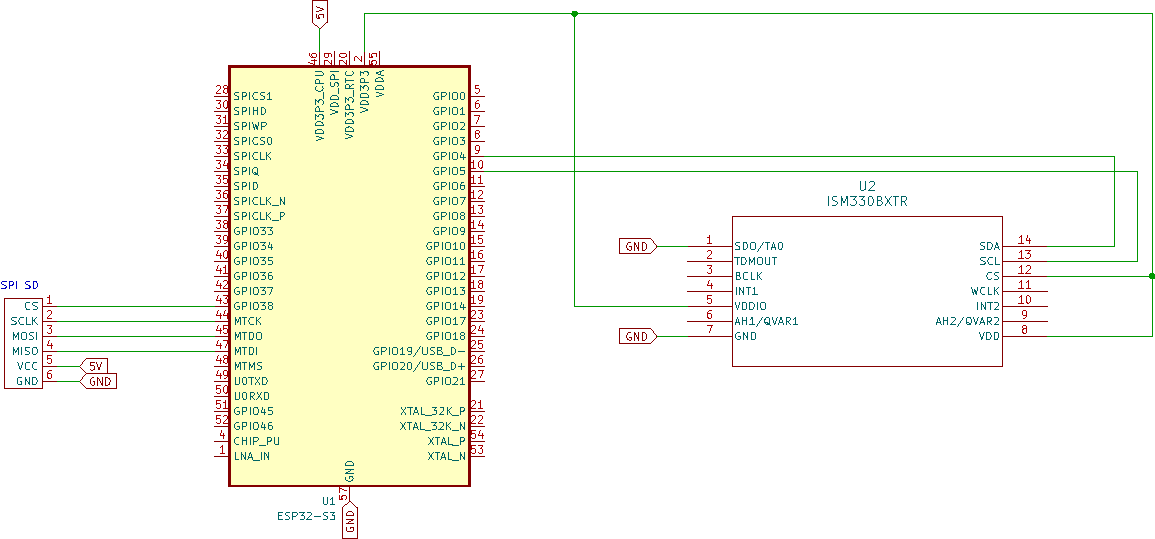
\includegraphics[width=0.95\textheight, height=0.8\textwidth, keepaspectratio]{assets/images/schematic.pdf}
	\caption{Schema logico}
	\label{fig:fullpage-schematic}
\end{sidewaysfigure}
\clearpage

\subsection{Consumo Energetico}

\begin{samepage}
\subsubsection{ESP32-S3 (Microcontrollore)}
\begin{table}[H]
	\centering
	\caption{ESP32-S3 Power Consumption -- CPU Active, \(25\,^\circ\mathrm{C}\)}
	\label{tab:esp32s3_cpu_power}
	\begin{tabularx}{\textwidth}{lccc}
		\hline
		\textbf{CPU Frequency} & \textbf{Peripherals} & \textbf{Data Access} & \textbf{Consumption} \\
		\hline
		$80\,\text{MHz}$  & $\times$     & $32$ bit  & $33.1\,\text{mA}$ \\
		$80\,\text{MHz}$  & \checkmark   & $32$ bit  & $47.3\,\text{mA}$ \\
		$80\,\text{MHz}$  & $\times$     & $128$ bit & $41.8\,\text{mA}$ \\
		$80\,\text{MHz}$  & \checkmark   & $128$ bit & $56.3\,\text{mA}$ \\
		$240\,\text{MHz}$ & $\times$     & $32$ bit  & $66.2\,\text{mA}$ \\
		$240\,\text{MHz}$ & \checkmark   & $32$ bit  & $81.3\,\text{mA}$ \\
		$240\,\text{MHz}$ & $\times$     & $128$ bit & $91.7\,\text{mA}$ \\
		$240\,\text{MHz}$ & \checkmark   & $128$ bit & $107.9\,\text{mA}$ \\
		\hline
	\end{tabularx}
\end{table}
\begin{table}[H]
	\centering
	\caption{ESP32-S3 Low-Power Modes, \(25\,^\circ\mathrm{C}\)}
	\label{tab:esp32s3_low_power}
	\begin{tabularx}{\textwidth}{lXc}
		\hline
		\textbf{Mode} & \textbf{Condition} & \textbf{Consumption} \\
		\hline
		Light-sleep & CPU e digital peripherals in clock-gating, Wi-Fi disattivato & $0.240\,\text{mA}$ \\
		Deep-sleep & RTC memory e RTC peripherals alimentati & $0.008\,\text{mA}$ \\
		\hline
	\end{tabularx}
\end{table}
\begin{table}[H]
	\centering
	\caption{ESP32-S3 Wi-Fi Power Consumption, \(25\,^\circ\mathrm{C}\)}
	\label{tab:esp32s3_wifi_power}
	\begin{tabularx}{\textwidth}{lXc}
		\hline
		\textbf{Mode} & \textbf{Configuration} & \textbf{Consumption} \\
		\hline
		Transmitter & $802.11\text{b}$, $1\,\text{Mbps}$, $P_{\text{OUT}}=+21\,\text{dBm}$ & $340\,\text{mA}$ \\
		Transmitter & $802.11\text{g}$, $54\,\text{Mbps}$, $P_{\text{OUT}}=+19\,\text{dBm}$ & $291\,\text{mA}$ \\
		Transmitter & $802.11\text{n}$, HT20, MCS7, $P_{\text{OUT}}=+18.5\,\text{dBm}$ & $283\,\text{mA}$ \\
		Transmitter & $802.11\text{n}$, HT40, MCS7, $P_{\text{OUT}}=+18\,\text{dBm}$ & $286\,\text{mA}$ \\
		Receiver & $802.11\text{b/g/n}$, HT20 & $88\,\text{mA}$ \\
		Receiver & $802.11\text{n}$, HT40 & $91\,\text{mA}$ \\
		\hline
	\end{tabularx}
\end{table}
\end{samepage}
Il profilo energetico usato é \textit{Modem-sleep mode}, rilasciato da Espressif \cite{esp32s3_datasheet}, dove il modem viene attivato solo quando necessario, quindi il consumo effettivo é:
\begin{itemize}
	\item in \textbf{Modem TX}: CPU Active/All RTC/Wi-Fi, durante la comunicazione dei dati (286 mA).
	\item in \textbf{Modem RX}: CPU Active/All RTC/Wi-Fi, durante la ricezione di modelli, comandi e configurazioni dei dati (91 mA).
	\item in \textbf{Modem sleep}: CPU Active/All RTC/No Wi-Fi, durante la fase di sola inferenza, scrittura su sd o lettura del sensore (81.3 mA).
\end{itemize}

Il sistema acquisisce campioni da \(12\,\mathrm{byte}\) (16bit per valore, 3 per accelerometro e 3 per giroscopio) ad una frequenza di
\(3.84\,\mathrm{kHz}\) (\(46.08\,\mathrm{kB/s}\)). I dati, convertiti in \textit{float32} (\(24\,\mathrm{byte}\) per campione), vengono trasmessi in blocchi da \(4096\) campioni.
La dimensione di ciascun blocco è quindi

\begin{equation}
	N_{\mathrm{TX}} = 4096 \cdot 24 = 98304\,\mathrm{byte}.
\end{equation}

Il periodo tra due trasmissioni in modalità \textit{continua}, ovvero vengono caricati tutti i \textit{datapoint}

\begin{equation}
	T_{\mathrm{block}} =
	\frac{4096}{3840}
	= 1.067\,\mathrm{s}.
\end{equation}

Assumendo la velocità teorica massima di \(150\,\mathrm{Mbit/s}\) per
802.11n HT40 MCS7, il tempo necessario per un blocco è

\begin{equation}
	T_{\mathrm{TX}} =
	\frac{98304\cdot8}{150\cdot10^6}
	= 5.24\,\mathrm{ms}.
\end{equation}

Assumendo una corrente di \(286\,\mathrm{mA}\) la potenza per singola trasmissione è

\begin{equation}
	E_{\mathrm{TX}}
	=
	\frac{3.3\cdot0.286\cdot5.24\times10^{-3}}{3.6}
	\approx
	\boxed{1.37\times10^{-3}\,\mathrm{mWh}}.
\end{equation}

Il duty cycle della trasmissione è

\begin{equation}
	D_{\mathrm{TX}} =
	\frac{5.24\,\mathrm{ms}}{1.067\,\mathrm{s}}
	\approx0.492\%.
\end{equation}

La corrente media associata al Wi-Fi è quindi

\begin{equation}
	I_{\mathrm{WiFi,avg}}
	=
	286\,\mathrm{mA}\cdot0.00492
	\approx1.41\,\mathrm{mA}.
\end{equation}

Considerando inoltre \(81.3\,\mathrm{mA}\) per CPU e periferiche attive, la corrente media complessiva risulta

\begin{equation}
	I_{\mathrm{avg}}
	=
	81.3+1.41
	\approx82.7\,\mathrm{mA}.
\end{equation}


I valori ottenuti rappresentano una stima teorica basata sulla velocità massima di \(150\,\mathrm{Mbit/s}\) e non tengono conto degli overhead del protocollo Wi-Fi e dei livelli superiori.


\begin{samepage}
\subsubsection{ISM330BX}

\begin{table}[H]
	\centering
	\small
	\begin{tabularx}{\textwidth}{l X r}
		\toprule
		\textbf{Modalità Operativa} & \textbf{Dettagli Canali e Funzionalità} & \textbf{Corrente Tipica ($I_{DD}$)} \\
		\midrule
		Combo High-Performance & Accelerometro + Giroscopio attivi ad alto ODR & $\approx \SI{0.60}{\milli\ampere}$ ($\SI{600}{\micro\ampere}$) \\
		Power-Down & Dispositivo spento, interfacce seriali in attesa & $\SI{3}{\micro\ampere}$ -- $\SI{5}{\micro\ampere}$ \\
		\bottomrule
	\end{tabularx}
	\caption{Consumi elettrici ISM330BX \cite{ism330bx_datasheet}.}
	\label{tab:ism330bx_power}
\end{table}
Il sensore viene usato in modalità \textit{High-Performance} a 3.84khz, con coda FIFO, ovvero il sensore salva in una regione di memoria le letture, il che permette di leggere a blocchi i dati dal sensore. Il firmware interroga il sensore chiedendo 512 byte alla volta.
\end{samepage}
\begin{samepage}

 \subsubsection{Adafruit 4682}
 Il breakout Adafruit 4682 è una scheda passiva, quindi il consumo é dato unicamente dalla scelta della scheda microsd.
Consumo scheda SD:
\begin{table}[H]
	\centering

	\label{tab:microsd-current}
	\begin{tabular}{lllcc}
		\hline
		Current &  $V_{\mathrm{DD}}$ & Max. \\
		\hline
		Peak
		& 3.6 V
		& 300 mA \\
		\hline
		Average
		& 3.6 V
		& 250 mA \\
		\hline
	\end{tabular}
		\caption{consumi di una scheda microSD, microSDXC, Class 10, U1, 64GB, modello SDCIT/64GB, marca Kingston \cite{kingston_industrial_microsd}.}
\end{table}

\end{samepage}


Analogamente al caso precedente, si riutilizzano gli stessi risultati per il
consumo del controllore. Considerando un data rate di
\(46.08\,\mathrm{kB/s}\), e una velocità minima di scrittura di
\(10\,\mathrm{MB/s}\) per una SD Classe 10, il duty cycle della scrittura o lettura è
pari a circa \(0.46\%\).

Assumendo un consumo di \(250\,\mathrm{mA}\) durante la scrittura o lettura il consumo
medio della SD è quindi circa \(1.15\,\mathrm{mA}\). Sommando il consumo
della CPU e delle periferiche, pari a \(81.3\,\mathrm{mA}\), si ottiene

\begin{equation}
	I_{\mathrm{avg,SD}}\approx82.45\,\mathrm{mA},
	\qquad
	P_{\mathrm{avg,SD}}\approx\boxed{272.1\,\mathrm{mW}}.
\end{equation}

\needspace{5\baselineskip}
\subsection{Sintesi dei Consumi di Sistema}
Sommando i consumi si ha un consumo medio teorico di $\approx83.75\mathrm{mA}$, o $\approx276.4\mathrm{mW}$, e un consumo di picco di $\approx 618.9\mathrm{mA}$ o $\approx2042\mathrm{mW}$.

Il che significa che una batteria 18650 da circa 9Wh, riuscirebbe ad alimentare il dispositivo per 32 ore.

\subsubsection{Tecniche di Ottimizzazione energetica}
La stima di 32 ore si riferisce all'autonomia con il massimo consumo, ovvero con continua lettura, salvataggio, invio dei dati e l'inferenza basata su suddetti dati.
Una volta che la \textit{backend} riceve abbastanza dati per allenare modelli validi si può mettere il device in varie modalità risparmio energetico configurabile. %circa lo supporta ma non proprio


\begin{table}[H]
	\centering
	\label{tab:esp32s3_duty_cycle}
	\begin{tabularx}{\textwidth}{lccccc}
		\hline
		\textbf{Modalità} & \textbf{CPU} & \textbf{Duty Cycle} & \textbf{Corrente} & \textbf{Potenza} & \textbf{Autonomia} \\
		\hline
		Active & $240\,\mathrm{MHz}$ & $100\%$ & $83.75\,\mathrm{mA}$ & $276.4\,\mathrm{mW}$ & $32.6\,\mathrm{h}$ \\
		Active & $80\,\mathrm{MHz}$ & $100\%$ & $49.75\,\mathrm{mA}$ & $164.2\,\mathrm{mW}$ & $54.8\,\mathrm{h}$ \\
		Light-sleep & $240\,\mathrm{MHz}$ & $3.33\%$ & $3.70\,\mathrm{mA}$ & $12.22\,\mathrm{mW}$ & $30.7\,\mathrm{giorni}$ \\
		Light-sleep & $80\,\mathrm{MHz}$ & $3.33\%$ & $2.57\,\mathrm{mA}$ & $8.48\,\mathrm{mW}$ & $44.2\,\mathrm{giorni}$ \\
		Deep-sleep & $240\,\mathrm{MHz}$ & $3.33\%$ & $3.48\,\mathrm{mA}$ & $11.47\,\mathrm{mW}$ & $32.7\,\mathrm{giorni}$ \\
		Deep-sleep & $80\,\mathrm{MHz}$ & $3.33\%$ & $2.34\,\mathrm{mA}$ & $7.74\,\mathrm{mW}$ & $48.5\,\mathrm{giorni}$ \\
		\hline
	\end{tabularx}
	\caption{Consumi e autonomia stimati nelle modalità, batteria da \(9\,\mathrm{Wh}\). Il duty cycle è del \(3.33\%\) (2 minuti di attività ogni ora, ovvero circa 112 segmenti da 4096 datapoint). Il duty cycle del Wi-Fi viene scalato a \(0.41\%\), il lettore SD è spento durante le fasi di sleep.}
\end{table}

\section{Software}
\subsection{Struttura principale}
Il codice del firmware é scritto in C/C++ usando il framework ESP-IDF.
Il sistema giova dell'architettura dual core del microcontrollore ESP32-S3 \cite{esp32s3_datasheet}.
Ci sono 6 task/thread principali.



\begin{table}[H]
	\centering
	\begin{tabularx}{\textwidth}{Xcc}
		\hline
		\textbf{Nome Task} & \textbf{Priorità} & \textbf{Core Assegnato} \\ \hline
		\texttt{harvester}   & 5                 & Core 1                  \\ \hline
		\texttt{inferencer}  & 4                 & Core 1                  \\ \hline
		\texttt{uploader}    & 3                 & Core 0                  \\ \hline
		\texttt{dump\_reader} & 3                 & Core 0                  \\ \hline
		\texttt{sd\_writer}   & 2                 & Core 0                  \\ \hline
		\texttt{mqtt\_task}  & 5 (Default)       & Core 0 (Default)        \\ \hline
	\end{tabularx}
	\caption{Priorità delle Task FreeRTOS e selezione Core}
	\label{tab:freertos_tasks}
\end{table}
Tutte le task nel core 0 hanno grandi ritardi di I/O perché richiedono chiamate di rete oppure la lettura e scrittura di file su scheda SD. Mentre l'inferencer nel Core 1 é cpu-bound per la maggior parte del tempo e IO-bound se deve caricare i modelli dalla rete oppure dalla scheda SD. L'harvester viene messo nello stesso Core dell'inferencer perché vogliamo dare precedenza alla lettura dei dati in maniera prioritaria.

\begin{description}
	\item[\texttt{harvester} (Core 1, Priorità 5)] Esegue l'interrogazione della coda FIFO del sensore ISM330BX via SPI per estrarre i campioni di accelerometro e giroscopio. La priorità é massima per permettere alla coda FIFO di non riempirsi mai e non andare in \textit{overrun} \cite{ism330bx_datasheet}, il che significherebbe perdere dei \textit{datapoints} contigui.

	\item[\texttt{inferencer} (Core 1, Priorità 4)] Calcola la magnitudo e carica dello spettrogramma STFT 2D. Esegue i modelli dell'\textit{ensemble} (insieme di modelli) e calcola il valore delle anomalie.

	\item[\texttt{uploader} (Core 0, Priorità 3)] Gestisce la serializzazione in formato CBOR e la trasmissione dei dati. Divide l'array di campioni float in pacchetti più piccoli per rientrare nei limiti dei buffer di rete dell'MQTT, e li invia al broker MQTT. %512 ma potrei cambiarlo


	\item[\texttt{dump\_reader} (Core 0, Priorità 3)] Viene istanziato temporaneamente in caso di trigger di replay, ovvero se la backend richiede un upload di tutti i dati storici salvati. Legge i file binari dalla scheda SD e li reinserisce nella pipeline di elaborazione, nello stesso modo in cui farebbe \textit{harvester}, che viene messo in pausa nel caso venga richiesto il replay. É un processo IO-bound, quindi messo nel Core 0.

	\item[\texttt{sd\_writer} (Core 0, Priorità 2)] Prende i dati (sia i datapoint che i risultati dell'inferenza) e li scrive sulla scheda SD in formato binario.

	\item[\texttt{mqtt\_task} (Core 0, Priorità 5 -- Default di Sistema)] Gestito in background dalla libreria client di MQTT di Espressif (\textit{espressif/mqtt} \cite{espressif_esp_mqtt}).
\end{description}

\subsection{4-way Buffer}
%citazione necessaria da trovare per il ping pong buffer.

La struttura dati principale che unisce le varie task é un \textit{4-way buffer}, una variante di un \textit{Ping Pong buffer} \cite{lyons2010dsp} con 4 buffer al posto di 2.
Tutte le task leggono e scrivono dagli slot del quad buffer, usando dei semafori per la sincronizzazione, e per evitare controlli attivi.

 \begin{figure}[H]
	\centering
	\begin{tikzpicture}[node distance=1.2cm, auto]

		\tikzstyle{state} = [draw=black, rectangle, rounded corners, minimum width=3.8cm, minimum height=1.2cm, align=center, thick, fill=white, font=\small]
		\tikzstyle{decision} = [draw=black, diamond, aspect=2, minimum width=3.8cm, minimum height=1cm, align=center, thick, fill=white, font=\small]
		\tikzstyle{flow} = [->, >=stealth, thick, draw=black]
		\tikzstyle{loopline} = [->, >=stealth, dashed, thick, draw=black!50]

		\node[state] (free) at (0,10.5) {\textbf{Slot Libero} };
		\node[state] (acq) at (0,8.6) {\textbf{Slot in Acquisizione} \\ \small (Preso da: \textbf{Harvester})};

		\node[decision] (dec) at (0,6.6) {Assegnamento slot};

		\node[state] (inf) at (-3.4,4.4) {\textbf{Slot in elaborazione} \\ \small (Acquisito da \textbf{Inferencer})};
		\node[state] (post_inf) at (-3.4,2.4) {\textbf{Slot elaborato}};

		\node[state] (bypass) at (3.4,3.4) {\textbf{Bypass elaborazione} \ };

		\node[state] (up_task) at (-2.4,-0.4) {\textbf{Slot pronto per Upload} \\ \small (Acquisito da \textbf{Uploader})};
		\node[state] (sd_task) at (2.4,-0.4) {\textbf{Slot pronto per SD} \\ \small (Acquisito da \textbf{SD Writer})};

		\draw[dashed, thick, black!70] (-5.4, 0.6) rectangle (5.4, -1.4);

		\node[font=\scriptsize\bfseries, black!70] at (0, 0.3) {ESECUZIONE CONCORRENTE };

		\node[state] (release) at (0,-3.2) {\textbf{Slot Rilasciato} };

		\draw[flow] (free) -- (acq);
		\draw[flow] (acq) -- (dec);

		\draw[flow] (dec.west) -| node[above, pos=0.5, font=\small] {Inferencer} (inf.north);
		\draw[flow] (dec.east) -| node[above, pos=0.5, font=\small] {Uploader \& SD} (bypass.north);

		\draw[flow] (inf) -- (post_inf);

		\coordinate (merge_point) at (0, 1.3);
		\coordinate (parallel_top) at (0, 0.6);

		\draw[thick] (post_inf.south) |- (merge_point);
		\draw[thick] (bypass.south) |- (merge_point);
		\draw[flow] (merge_point) -- (parallel_top);

		\draw[flow] (up_task.south) |- (release.west);
		\draw[flow] (sd_task.south) |- (release.east);

		\draw[loopline] (release.south) -- ++(0,-0.8) -- ++(-6.8,0) |- node[left, pos=0.9, font=\scriptsize, align=center] {Reinserito in\\free\_slots\_queue} (free.west);

	\end{tikzpicture}
	\caption{Grafo del ciclo di vita di uno slot in modalità continua}
	\label{fig:slot_lifecycle_fork_join_spaced}
\end{figure}


L'harvester prende il primo slot che trova quindi, dopo essere stato popolato dai dati, viene acquisito dall'inferencer, e poi sd\_writer e uploader salvano su sd e caricano sul cloud il segmento con i dati inferenziali ,oppure se l'inferencer sta elaborando un altro slot, viene assegnato direttamente al uploader e al sd\_writer, che salvano e caricano lo slot senza dati inferenziali.
La ragione per cui abbiamo bisogno di 4 buffer é che questo garantisce che 2 siano sempre occupati dal harvester che salva i dati come un classico ping pong buffer senza interruzioni, uno sia occupato dall'inferencer e un altro dai uploader e sd\_writer, in questo modo nessun task deve aspettarne un altro.

Il sistema é predisposto anche per altre modalità. Le modalità di upload di dati, configurabili dalla backend runtime sono:

\begin{itemize}
	\item \textit{Continuous}: ovvero quello nel grafico sopra, il device carica sul cloud tutti i dati che riesce, elaborati o no.
	\item \textit{AnomalyOnly}: il device carica sul cloud il segmento solo se risulta in un anomalia.
	\item \textit{AnomalyOrPeriodic}: il device carica sul cloud il segmento solo se risulta in un anomalia, ma carica con una certa cadenza anche dati non anomali per permettere un allenamento continuo dei modelli.
	\item \textit{ContinuousScoreRawAnomaly}: il device carica sempre il risultato dell'inferenza, ma carica anche il segmento solo se si tratta di un anomalia.
\end{itemize}

Il device espone alla backend dei comandi di dump opzionali, questi sono \textit{dump}, che carica sul cloud tutti i dati dalla scheda SD senza farne l'inferenza (harvester e inferencer disabilitati) e \textit{dump\_i} che carica tutti i dati, ma calcolandone anche le anomalie (harvester disabilitato).

Nella configurazione del device é possibile anche disabilitare del tutto la scheda sd per risparmiare energia se non si ha bisogno di chiamare il comando \textit{dump} dei dati.

\section{Inferencer}
L'inferencer è la task che gestisce la vita dei modelli e la loro inferenza, appoggiandosi ad una struttura dati chiamata \textit{ensemble} che aiuta la gestione dei modelli e astrae l'utilizzo della libreria tflite micro \cite{espressif_esp_tflite_micro}.
Ai dati viene applicata una pipeline che riduce la dimensionalità, ovvero una riduzione euclidea di magnitudo per accelerazione e giroscopio:

\begin{samepage}

$$\text{Accel Magnitude}[n] = \sqrt{\text{accel}_x[n]^2 + \text{accel}_y[n]^2 + \text{accel}_z[n]^2}$$

$$\text{Gyro Magnitude}[n] = \sqrt{\text{gyro}_x[n]^2 + \text{gyro}_y[n]^2 + \text{gyro}_z[n]^2}$$
\end{samepage}
questo permette di mantenere solo i dati vibrazionali, indipendentemente dall'orientamento di montaggio del sensore.

Successivamente viene applicata ad entrambi una funzione a finestra di hanning (overlap 75\%) e una trasformazione di Fourier.
Viene scelta la finestra di Hanning perchè offre un buon compromesso tra risoluzione e contenimento dello spectral leakage \cite{harris1978use}.


\begin{figure}
	\centering
	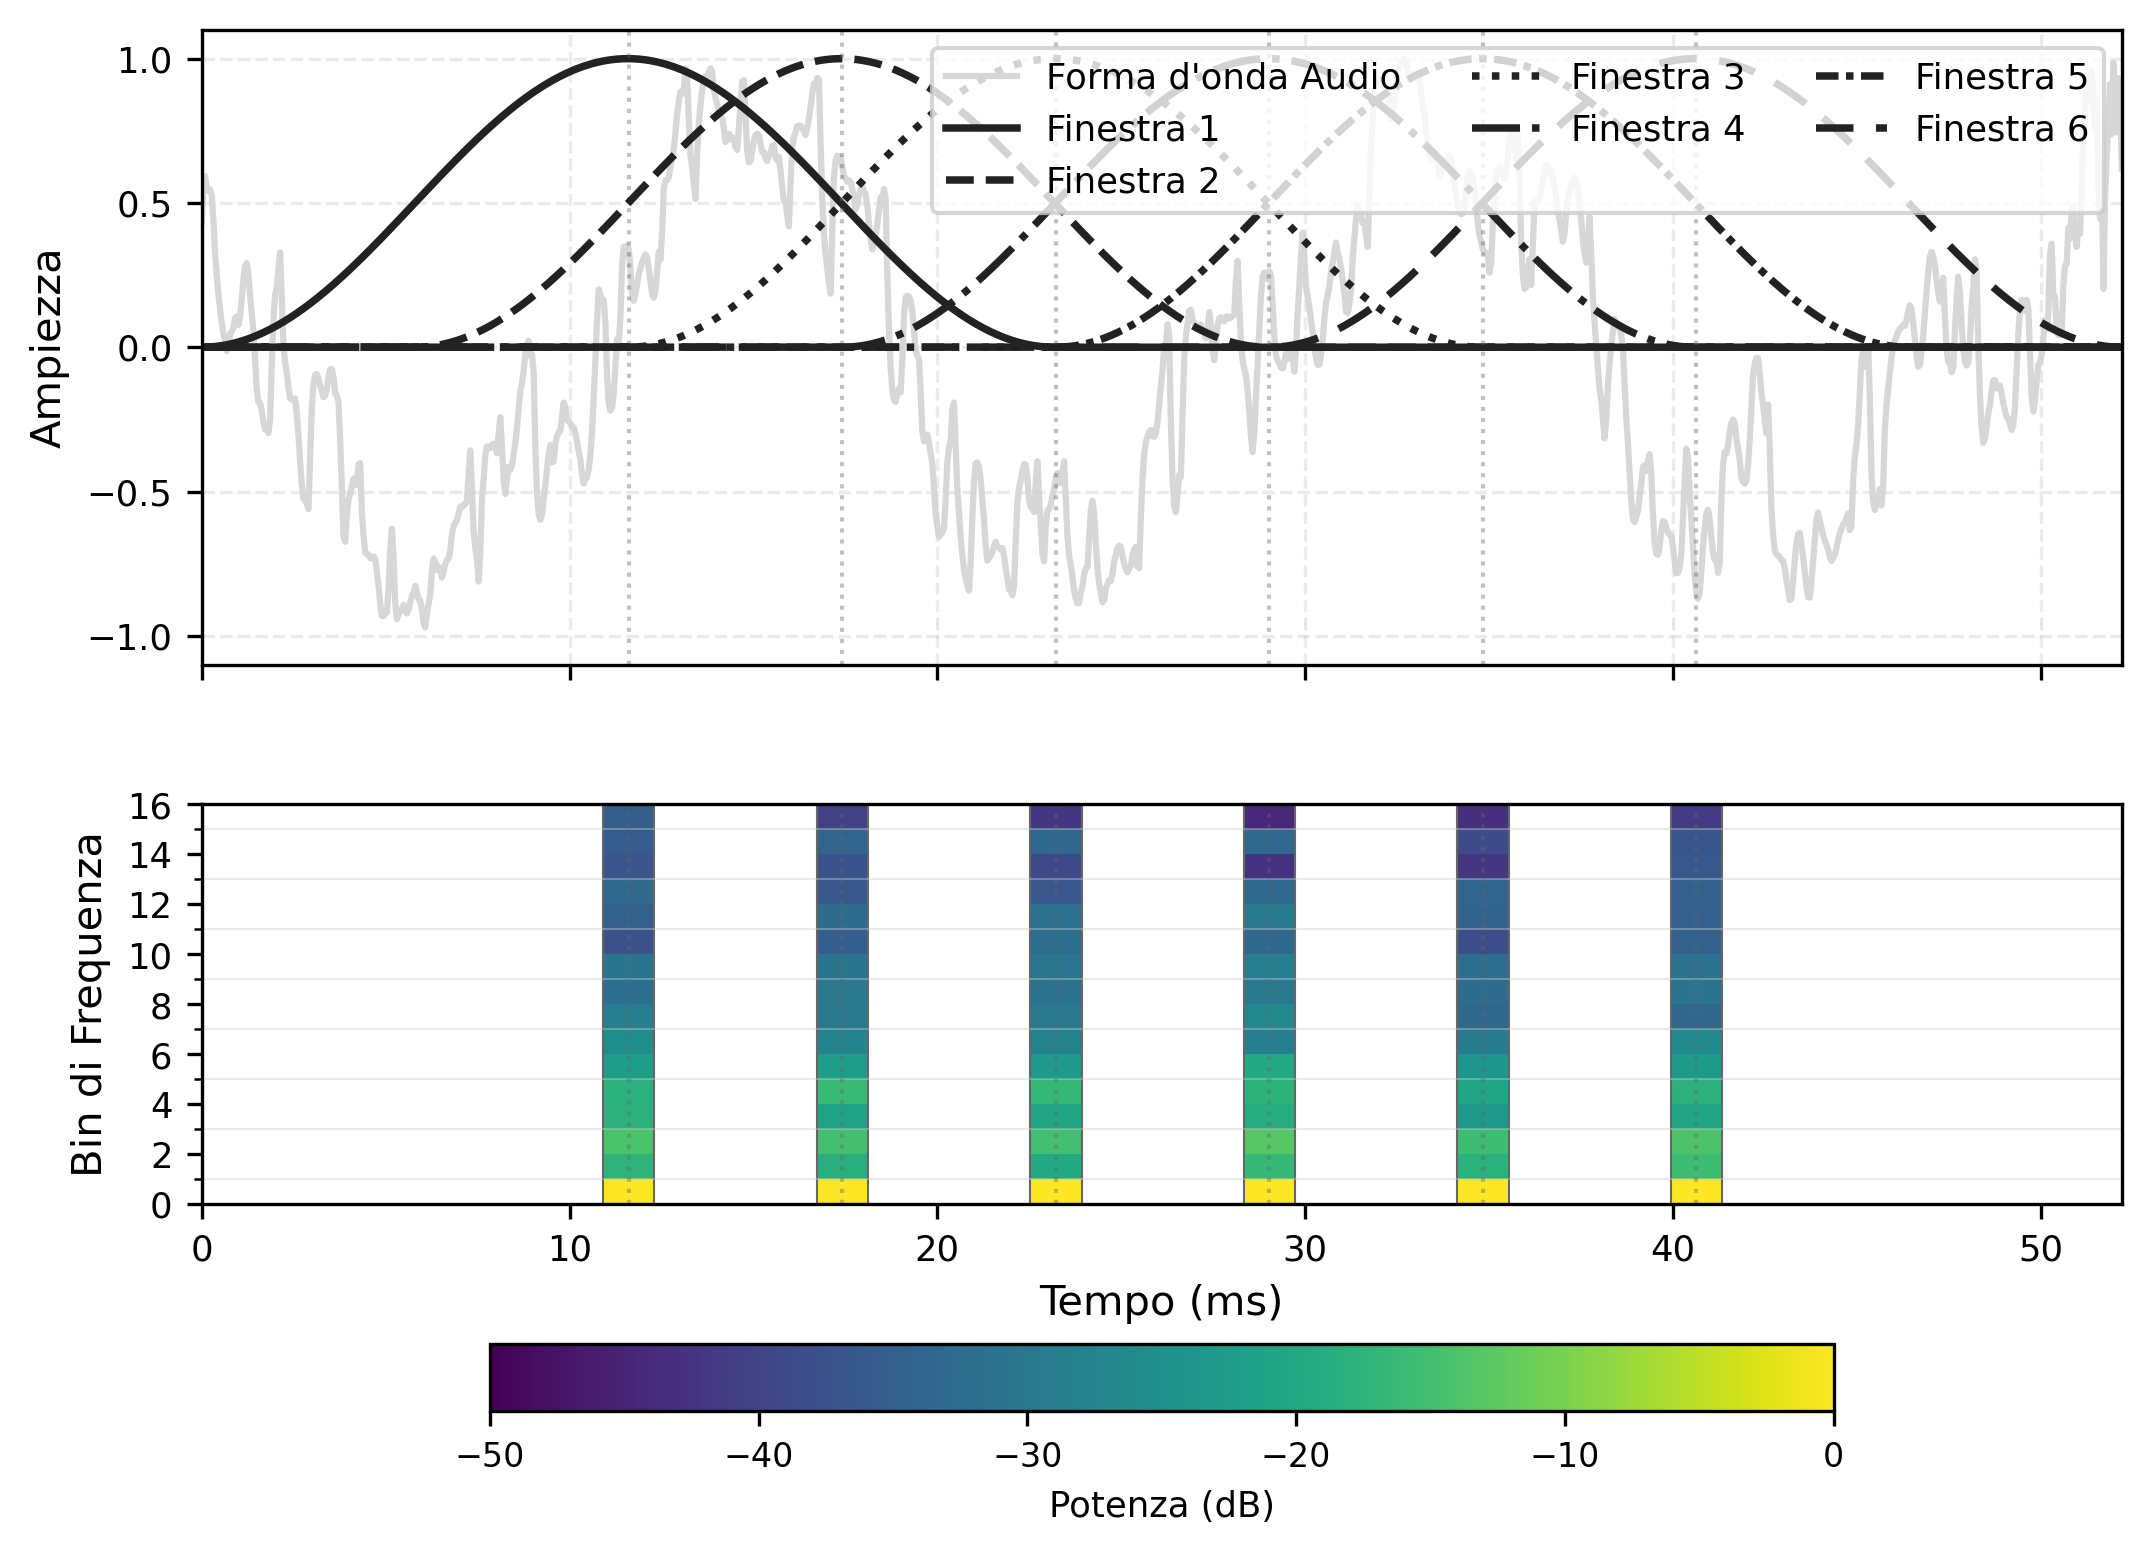
\includegraphics[width=1\linewidth]{assets/images/stft}
	\caption{Applicazione finestra di hanning e trasformata di fourier}
	\label{fig:stft}
\end{figure}

Infine gli spettrogrammi STFT del giroscopio e accelerazione vengono concatenati lungo l'asse delle feature di frequenza, così da creare un solo segmento di dati.

\subsection{Architettura dell'\textit{ensemble}}
L'architettura è formata da 3 tipi di modelli disposti in maniera simil-MIXAE \cite{mixae_zhang2017deep}:


\begin{figure}[H]
	\centering
	\resizebox{\textwidth}{!}{%
		\begin{tikzpicture}[
			>=Stealth,
			box/.style={
				draw,
				thick,
				fill=white,
				minimum width=2.4cm,
				minimum height=1.15cm,
				align=center,
				rounded corners=2pt,
				font=\sffamily
			},
			imgbox/.style={
				draw,
				thick,
				inner sep=0pt,
				fill=white
			},
			stackbox/.style={
				draw,
				thick,
				fill=white,
				minimum width=2cm,
				minimum height=2cm
			},
			solid arr/.style={
				thick,
				->,
				rounded corners=3pt
			},
			dashed arr/.style={
				dashed,
				thick,
				->,
				rounded corners=3pt
			},
			double line/.style={
				double,
				double distance=2pt,
				thick,
				rounded corners=3pt
			},
			font=\sffamily
			]

			% Input
			\coordinate (in_pos) at (0,0);

			\node[stackbox, shift={(-6pt,6pt)}] at (in_pos) {};
			\node[stackbox, shift={(-3pt,3pt)}] at (in_pos) {};

			\node[imgbox] (input) at (in_pos)
			{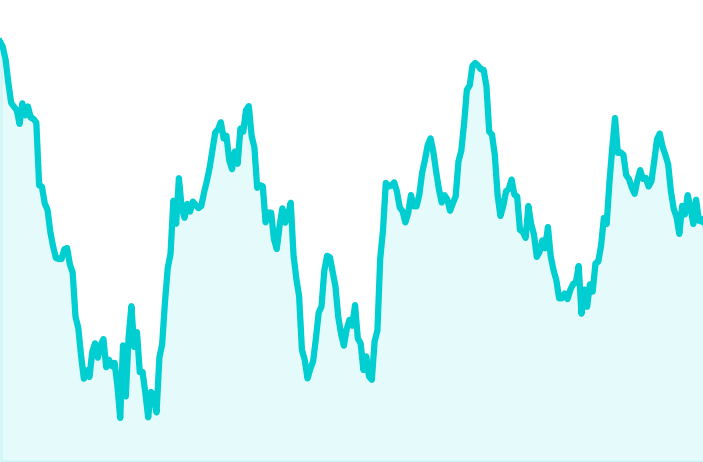
\includegraphics[
				width=2cm,
				height=2cm
				]{assets/images/waveform.png}};

			\node[below=0.15cm of input, font=\small] {Input};

			% STFT
			\node[imgbox] (stft) at (3.5,0)
			{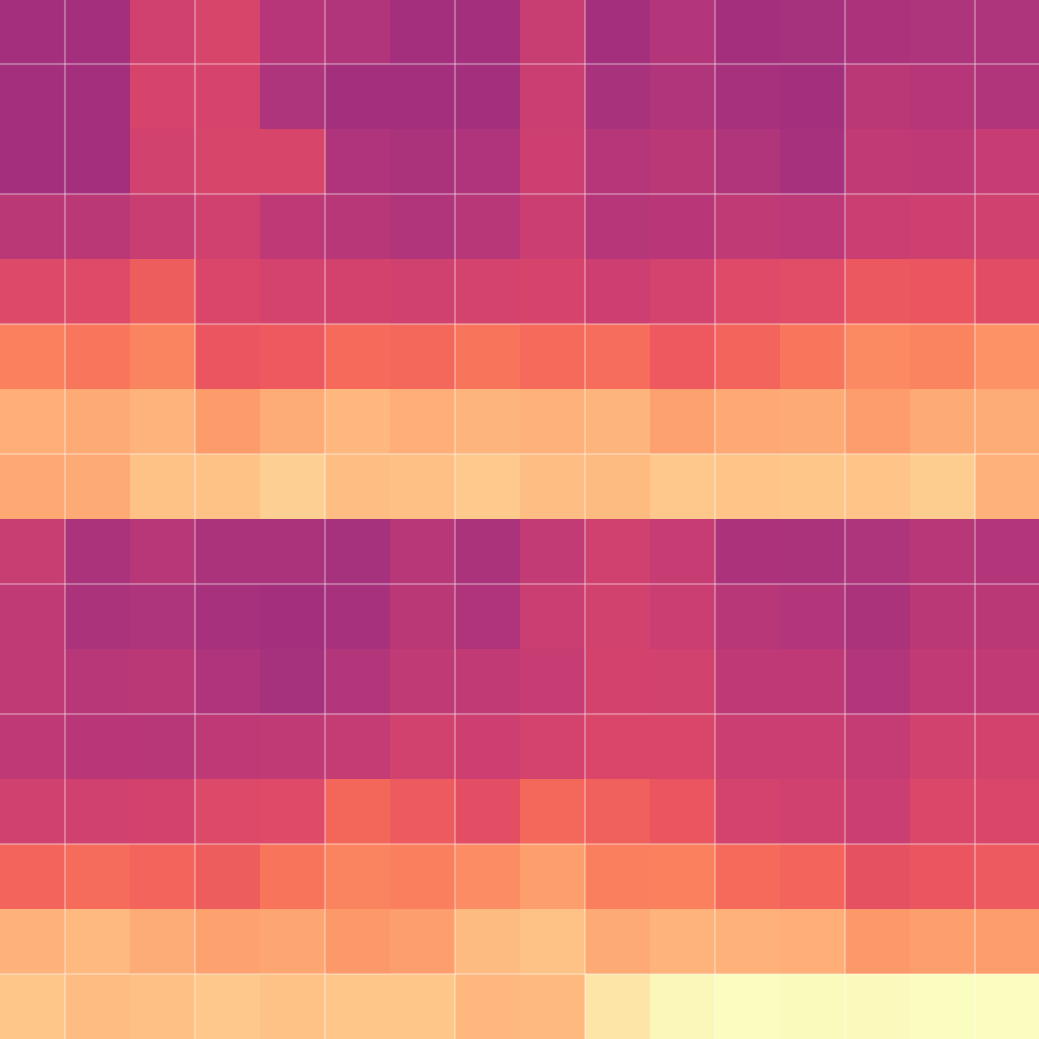
\includegraphics[
				width=2cm,
				height=2cm
				]{assets/images/spectrogram3.png}};

			\node[below=0.15cm of stft, font=\small] {STFT};

			\draw[solid arr]
			(input.east) -- (stft.west);

			% Router e Memoria
			\node[box] (router) at (7.0,1.6) {Router};
			\node[box] (memory) at (7.0,-1.6) {Memoria};

			% Split principale dopo STFT (Est)
			\coordinate (stft_split) at (5.2,0);

			\draw[thick]
			(stft.east) -- (stft_split);

			% STFT -> Router
			\draw[solid arr]
			(stft_split)
			-- (5.2,1.6)
			-- (router.west);

			% STFT -> Memoria
			\draw[solid arr]
			(stft_split)
			-- (5.2,-1.6)
			-- (memory.west);

			% Memoria -> Router (concat)
			\draw[dashed arr]
			(memory.north)
			-- (router.south)
			node[midway,right,font=\footnotesize] {concat};

			% Modelli
			\node[box] (mod1) at (12.5,1.6) {Modello 1};
			\node[font=\Huge] (dots) at (12.5,0) {$\vdots$};
			\node[box] (modN) at (12.5,-1.6) {Modello $N$};

			% Ingressi Modello 1: STFT (alto), Router (centro), Memoria (basso)
			\coordinate (m1_stft)   at (11.3,1.76);
			\coordinate (m1_router) at (11.3,1.60);
			\coordinate (m1_mem)    at (11.3,1.44);

			% Ingressi Modello N: STFT (alto), Memoria (centro), Router (basso)
			\coordinate (mN_stft)   at (11.3,-1.44);
			\coordinate (mN_mem)    at (11.3,-1.60);
			\coordinate (mN_router) at (11.3,-1.76);

			% Router -> modelli (Trunk a x=9.5)
			\coordinate (router_split) at (9.5,1.6);

			% Verso Modello 1 (dritto al centro: y=1.60)
			\draw[double line, ->]
			(router.east) -- (router_split) -- (m1_router);

			% Verso Modello N (scende alla porta inferiore: y=-1.76)
			\draw[double line, ->]
			(router.east) -- (router_split) |- (mN_router);

			% STFT -> Modelli e snstruction Error (percorso inferiore)
			\coordinate (model_recon_split) at (10.0,-4.2);

			% Da stft_split scende a -4.2 e va a destra fino allo split
			\draw[thick]
			(stft_split) -- (5.2,-4.2) -- (model_recon_split);

			% STFT -> Modello 1 (Porta superiore: y=1.76)
			\draw[solid arr]
			(model_recon_split)
			-- (10.0,1.76)
			-- (m1_stft);

			% STFT -> Modello N (Porta superiore: y=-1.44)
			\draw[solid arr]
			(model_recon_split)
			-- (10.0,-1.44)
			-- (mN_stft);

			% Memoria -> modelli (Trunk a x=10.5)
			% Linea perfettamente orizzontale da memory.east (y=-1.60) fino a x=10.5
			\coordinate (memory_split) at (10.5,-1.6);

			\draw[dashed,thick]
			(memory.east) -- (memory_split);

			% Da x=10.5 sale verso Modello 1 (Porta inferiore: y=1.44)
			\draw[dashed arr]
			(memory_split)
			-- (10.5,1.44)
			-- (m1_mem);

			% Da x=10.5 va dritto verso Modello N (Porta centrale: y=-1.60)
			\draw[dashed arr]
			(memory_split) -- (mN_mem);

			% Output
			\node[imgbox] (output) at (16.0,1.6)
			{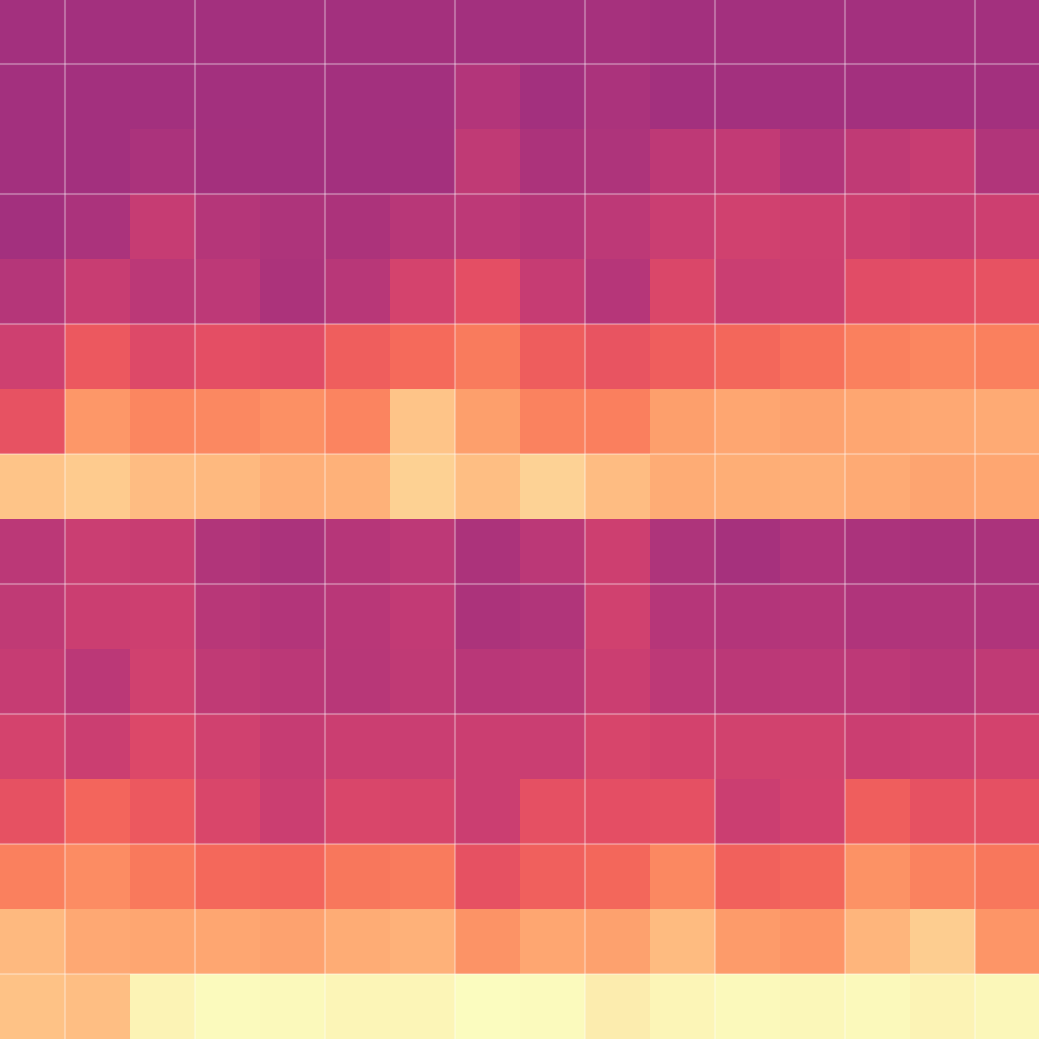
\includegraphics[
				width=2cm,
				height=2cm
				]{assets/images/spectrogram4.png}};

			\node[below=0.15cm of output, font=\small]
			{Output Selezionato};

			\draw[solid arr]
			(mod1.east) -- (output.west);

			% Reconstruction Error
			\node[
			box,
			fill=gray!10
			] (recon) at (16.0,-4.2)
			{Errore di \\ ricostruzione};

			% STFT -> Reconstruction Error (collegamento diretto orizzontale)
			\draw[solid arr]
			(model_recon_split) -- (recon.west);

			% Output -> Reconstruction Error
			\draw[solid arr]
			(output.south)
			-- (output.south |- recon.north)
			-- (recon.north);

			% Legenda
			\node[
			draw,
			thick,
			rounded corners=2pt,
			fill=white,
			align=left,
			inner sep=6pt,
			font=\footnotesize
			] at (7.5,-5.85)
			{%
				\textbf{Legenda}\\[3pt]
				\tikz[baseline=-0.5ex]
				\draw[thick,->] (0,0) -- (0.8,0);
				\quad Flusso principale\\[4pt]
				\tikz[baseline=-0.5ex]
				\draw[double,double distance=2pt,thick,->]
				(0,0) -- (0.8,0);
				\quad Selezione modello (argmax)\\[4pt]
				\tikz[baseline=-0.5ex]
				\draw[dashed,thick,->] (0,0) -- (0.8,0);
				\quad Memoria (opzionale)
			};

		\end{tikzpicture}%
	}
	\caption{Architettura del \textit{ensemble}.}
	\label{fig:architecture}
\end{figure}


\begin{itemize}
	\item 1 \textbf{Router}: prende in input un segmento e lo stato della memoria e decide quale autoencoder dovrà processarlo.
	\item 1 \textbf{Memoria}: memoria, opzionale per modello. Utile per modelli non convoluzionali, è un modo per aggiungere informazioni sul passato.
	\item N \textbf{autoencoder}: ci sono N (max 16), autoencoder che prendono il segmento e provano a ricostruirlo, l'errore di ricostruzione indica il livello di anomalia, configurabile tra MSE lineare e MSE logaritmico, può essere usato qualsiasi modelli rappresentabile con grafi nativi tflite micro.

\end{itemize}


\subsection{Gestione dei sottomodelli}
In memoria non possono alloggiare tutti i sottomodelli, se si scelgono architetture troppo complesse, quindi è necessario avere un modo di caricare a bisogno i sottomodelli.
Per questo l'inferencer dispone di una struttura dati di cache di modelli, creando così una gerarchia di recupero dati. Prima viene interrogata la cache alla ricerca del modello, poi la scheda sd se abilitata, poi il cloud attraverso una richiesta MQTT.
Una volta caricato un nuovo modello, se la memoria non è sufficiente, viene rimosso il modello usato meno recentemente, liberando così una parte di memoria.


% aggiungere sdw writer, harvester, uploader e dump_reader? non c'è tanto altro da dire

\section{Ottimizzazioni}
Vengono usate varie funzioni ottimizzate per l'ESP32S3.
\begin{itemize}
	\item \textbf{dsp\_opt\_int16\_to\_float}, custom, permette di convertire un buffer da int16
	a float con l'istruzione FLOAT.S di Xtensa LX7 \cite{xtensa_isa}.
	 \item \textbf{\texttt{dsps\_fft2r\_fc32} (Radix-2 Complex FFT)}: calcola la fft sui dati del sensore. Fornita da ESP-DSP \cite{espdsp}.
	\item \textbf{\texttt{dsps\_fft2r\_init\_fc32} (Inizializzazione FFT)}: Precalcola le tabelle dei fattori rotazionali (\textit{twiddle factors}) per evitare runtime calcoli di seni e coseni, molto pesanti. Fornita da ESP-DSP \cite{espdsp}.
	\item \textbf{\texttt{dsps\_bit\_rev\_fc32} (Bit Reversal)}: Esegue il riordinamento dell'array in output di dsps\_fft2r\_fc32. Fornita da ESP-DSP \cite{espdsp}.
	\item \textbf{\texttt{dsps\_wind\_hann\_f32} (Generazione Finestra di Hanning)}: Calcola e applica la finestra di Hann. Fornita da ESP-DSP \cite{espdsp}.
	\item \textbf{\texttt{dsps\_mulc\_f32} (Moltiplicazione Vettore-Scalare)}: Esegue la moltiplicazione di un array float per un numero. Fornita da ESP-DSP \cite{espdsp}.
\end{itemize}


\subsection{Ottimizzazione della conversione in float}
\label{subsec:dsp_optimization}
Il sensore restituisce dati in tipo int16, ma le funzioni di calcolo si aspettano dati in formato float da -1 a 1, quindi dobbiamo convertirli usando la funzione dsp\_opt\_int16\_to\_float che sfrutta l'istruzione assembly FLOAT.S.

\subsubsection{L'istruzione \texttt{FLOAT.S}}
L'approccio \textit{naive} sarebbe fare un ciclo for facendo un cast di ogni valore del buffer in float e poi moltiplicarlo per $1/32768.0$:
\begin{equation}
	x_{\text{float}} = \text{(float)}x_{\text{int16}} \cdot \frac{1}{32768.0}
\end{equation}
Questo approccio fa eseguire nell'FPU del controllore due istruzioni: un cast hardware (\texttt{FLOAT.S} con fattore di scala nullo) ed una moltiplicazione in floating point (\texttt{MUL.S}).

Per ottimizzare si è sfruttato l'ISA del coprocessore matematico dell'architettura Xtensa LX7 dell'ESP32-S3. Come scritto nel manuale dell'ISA \cite{xtensa_isa},
 \texttt{FLOAT.S} possiede un campo per fare lo shift del risultato:
\begin{equation}
	\text{FR}[r] \leftarrow \text{floats}(\text{AR}[s]) \cdot 2^{-t} \quad \text{con } t \in [0, 15]
\end{equation}
Impostando $t = 15$, la FPU procede col casting int16-float e la divisione per $2^{15} = 32768$ nello stesso ciclo di clock. Si
elimina così l'istruzione di moltiplicazione e l'overhead di memoria per la costante.

\subsubsection{Ottimizzazione della pipeline}
Come definito nei modelli di schedulazione di GCC per l'architettura
Xtensa \cite{gcc_xtensa}, le istruzioni di caricamento sulla memoria \texttt{load} e di conversione (\texttt{fconv}) hanno latenze:
\begin{itemize}
	\item \textbf{Caricamento (\texttt{xtensa\_memory})}: 2 cicli di clock.
	\item \textbf{Conversione (\texttt{xtensa\_fconv})}: 2 cicli di clock (fully-pipelined, con throughput di 1 istruzione per ciclo).
\end{itemize}
Quindi se viene eseguita la conversione con FLOAT.S elemento per elemento, ovvero con fattore di unrolling U=1, la cpu dovrà continuare ad aspettare che la FPU scriva i risultati nei registri prima di poter salvare il valore in memoria.
Per evitare la latenza di pipeline abbiamo bisogno di un fattore di unrolling U maggiore uguale della latenza di pipeline \cite{patterson_hennessy}.

La latenza che abbiamo è di 4 cicli (2 di caricamento+2 di conversione), Quindi scegliamo U=4.


Lo pseudocodice dell'algoritmo ottimizzato con inline assembly è riportato nel Codice \ref{lst:dsp_opt_s3_assembly}.
\begin{lstlisting}[
	language=C,
	caption={Algoritmo di conversione ottimizzato a 4 vie con assembly Xtensa},
	label=lst:dsp_opt_s3_assembly,
	frame=single,
	basicstyle=\small\ttfamily,
	keywordstyle=\color{blue},
	commentstyle=\color{gray},
	breaklines=true,
	tabsize=2,
	keepspaces=true
	]
	void dsp_opt_int16_to_float(const int16_t *src, float *dest,
			int len) {
		int i = 0;
		for (; i + 3 < len; i += 4) {
			// genera istruzioni L16SI,
			// carica e converte in 2 cicli
			int32_t s0 = src[i+0]; int32_t s1 = src[i+1];
			int32_t s2 = src[i+2]; int32_t s3 = src[i+3];
			float f0, f1, f2, f3;

			asm volatile (
			"float.s %[f0], %[s0], 15 \n\t"
			"float.s %[f1], %[s1], 15 \n\t"
			"float.s %[f2], %[s2], 15 \n\t"
			"float.s %[f3], %[s3], 15"
			: [f0] "=f" (f0), [f1] "=f" (f1), [f2] "=f" (f2),
					[f3] "=f" (f3)
			: [s0] "r" (s0), [s1] "r" (s1), [s2] "r" (s2),
					[s3] "r" (s3)
			);

			dest[i+0] = f0; dest[i+1] = f1;
			dest[i+2] = f2; dest[i+3] = f3;
		}
	}
\end{lstlisting}

\subsubsection{Validazione sperimentale benchmark}
Per validare l'analisi è stato condotto un benchmark sull'ESP32-S3 misurando i cicli di clock effettivi tramite il registro \texttt{CCOUNT}.
Ogni benchmark è stato fatto su 20000 volte un buffer da 4096 valori, per simulare il vero utilizzo.


\begin{table}[H]
	\centering
	\begin{tabular}{lcccc}
		\toprule
		\textbf{Configurazione} & \textbf{Cicli/op} & \textbf{Tempo buffer} & \textbf{Ottimizzazione} & \textbf{Speedup} \\
		\midrule
		Assembly x1  & 17.08 & $291.50\,\mu\text{s}$ & $29.24\%$ & $1.41\times$ \\
		Assembly x2  & 10.57 & $180.39\,\mu\text{s}$ & $56.21\%$ & $2.28\times$ \\
		\textbf{Assembly x4} & \textbf{8.26} & $\mathbf{140.97\,\mu\text{s}}$ & $\mathbf{65.78\%}$ & $\mathbf{2.92\times}$ \\
		Assembly x8  &  9.01 & $153.77\,\mu\text{s}$ & $62.68\%$ & $2.68\times$ \\
		\midrule
		Naive C x1   & 24.14 & $411.99\,\mu\text{s}$ & $0.00\%$  & $1.00\times$ \\
		Naive C x2   & 17.58 & $300.03\,\mu\text{s}$ & $27.17\%$ & $1.37\times$ \\
		Naive C x4   & 14.32 & $244.39\,\mu\text{s}$ & $40.68\%$ & $1.68\times$ \\
		Naive C x8   & 12.82 & $218.79\,\mu\text{s}$ & $46.90\%$ & $1.88\times$ \\
		Naive C x16  & 11.95 & $203.95\,\mu\text{s}$ & $50.50\%$ & $2.02\times$ \\
		Naive C x32  & 22.55 & $384.85\,\mu\text{s}$ & $6.59\%$  & $1.07\times$ \\
		Naive C x64  & 23.34 & $398.29\,\mu\text{s}$ & $3.33\%$  & $1.03\times$ \\
		\bottomrule
	\end{tabular}
	\caption{Risultati del benchmark su ESP32-S3 a 240 MHz}
	\label{tab:fpu_benchmark_results}
\end{table}

Si può notare che il metodo più veloce è Assembly con U=4, il che conferma l'analisi teorica.
Si può anche notare che il metodo naive più veloce è con U=16, questo perchè la pipeline di calcolo naive è lunga 9 cicli perchè viene scomposta in 4 istruzioni, ovvero L16SI (2 cicli), FLOAT.S (2 cicli, senza shift), MUL.S (4 cicli), SSI (Store Single Precision, 1 ciclo), per un totale di 9 cicli totali. U deve essere quindi maggiore o uguale a 9, tuttavia per allineamento alla dimensione del bus, usiamo la potenza di due maggiore più vicina, ovvero 16.




\newpage
\chapter{Modelli utilizzati}
%troppo poco come introduzione? o inutile?
Come abbiamo detto ci sono 3 tipi di modelli, il modello memoria, il modello router, e N sottomodelli autoencoder.

\subsection{Modello Memoria}
\begin{tikzpicture}[
	node distance=2cm,
	box/.style={
		draw,
		thick,
		rectangle,
		minimum width=1.5cm,
		minimum height=4.5cm,
		align=center
	},
	arrow/.style={-Latex, thick}
	]
	
	% Nodi
	\node[align=center] (input) {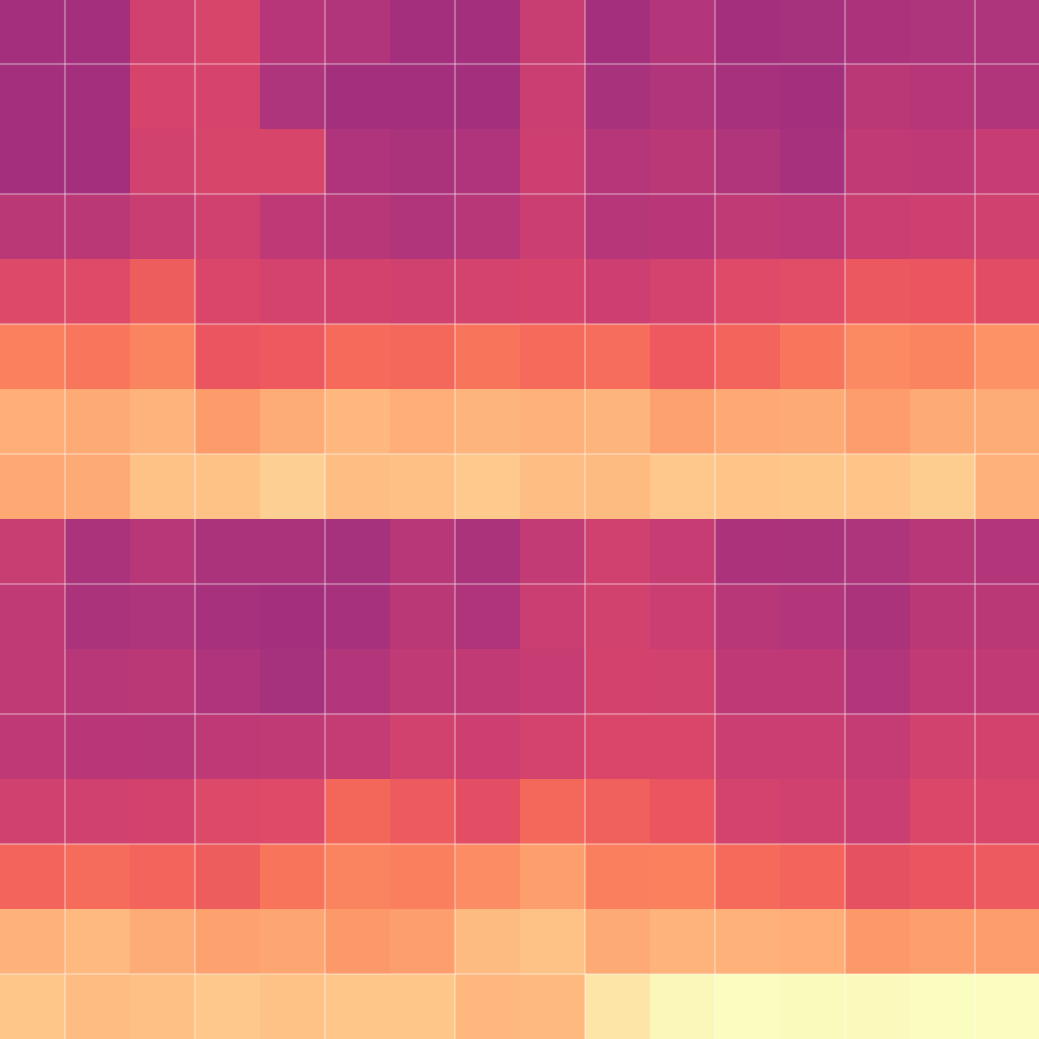
\includegraphics[height=2.5cm]{assets/images/spectrogram3.png}\\[0.2cm] Input};
	\node[box, right=of input] (lstm1) {\rotatebox{90}{LSTM Layer 1}};
	\node[box, right=of lstm1] (lstm2) {\rotatebox{90}{LSTM Layer 2}};
	\node[box, right=of lstm2] (output) {\rotatebox{90}{Output ($h_t$)}};
	
	% Connessioni lineari
	\draw[arrow] (input) -- (lstm1);
	\draw[arrow] (lstm1) -- (lstm2);
	\draw[arrow] (lstm2) -- (output);
	
	% Connessioni ricorrenti
	\path[arrow] (lstm1.north east) edge[out=70, in=110, looseness=3] node[above, font=\scriptsize] {Stato} (lstm1.north west);
	\path[arrow] (lstm2.north east) edge[out=70, in=110, looseness=3] node[above, font=\scriptsize] {Stato} (lstm2.north west);
	
\end{tikzpicture}

                       
	 \textbf{LSTM Memory Backbone} utilizza dei layer a Long Short Term Memory (LSTM) \cite{hochreiter1997lstm}, che permettono agli altri sottomodelli dicordare dati passati. Riceve in input i singoli segmenti dello spettrogramma e fornisce in output una rappresentazione latente dei dati. % ora che ci penso dovrei mettere controlli in caso di EGVG
	 Il modello memoria é condiviso con tutti i modelli che lo usano, quindi gli altri modelli devono essere allenati dopo il modello memoria.

\subsubsection{Modello router}                                                                                                                                                                                  
Il Router classifica i dati per selezionare l'autoencoder idoneo.                                                                                                                                
Le architetture usate sono:
\begin{enumerate}                                                                                                                                                                                                                    
	\item \textbf{Fully connected}:                                                                                                                                                                 
Rete neurale densa (Multilayer Perceptron, MLP) %altro da dire?              

	\item \textbf{STFT MCNN}:                                                                                                                                                           
Multi-branch Convolutional Neural Network. Applica reti convoluzionali parallele per estrarre caratteristiche dei dati diverse, usando kernel di dimensioni diverse \cite{zhang2016mcnn}.                                                                                                                                                        
         
	
	\item \textbf{1D CNN}
	Rete convoluzionale (multilivello) ad un kernel per livello che scansiona lo spettrogramma, ha un MLP finale per la classificazione.                                                                 
\cite{kiranyaz20151dcnn}
\end{enumerate}                                                                                                                                                                                                                      
\subsubsection{Modelli autoencoder}                       
%troppo prolisso/confuso?
Provano a ricostruire il segnale di input, la ragione per cui sono utili nel contesto dell'anomaly detection è che riescono a ricostruire il segnale di input solo se sono stati allenati con dati i a quelli che dovranno poi ricostruire, questo fa si che se incontrano dati mai visti non riusciranno a ricostruire in maniera affidabile l'input, e quindi possiamo assumere che quell'input è diverso in struttura dai dati in cui è stato allenato.

%TODO aggiungere disegno esplicativo di un AE?
\begin{enumerate}                                                                                                                                                     
	\item  \textbf{Autoencoder denso}:
	Usa semplici layer densi, essendo di fatto un MLP con dei layer di bottleneck, che formano lo spazio latente, tra l'encoder e il decoder
	
	\item \textbf{Variational
		autoencoder}:
		% si capisce? troppo corto
		Un VAE è, a livello strutturale, un autoencoder denso, tuttavia nella fase di training, si forza lo spazio latente ad essere formato da una distribuzione normale   $\mathcal{N}(0, 1)$ di $\mathcal{N}$ dimensioni. Questo permette allo spazio latente di non avere buchi, ovvero zone che producono in fase di decode dati incoerenti \cite{kingma2013auto}.
		
		
	\item \textbf{Convolutional Autoencoder 1D}:
	Usa layer convoluzionali in fase di encode, e layer deconvoluzionali in fase di decode. Utilizza come input lo spettrogramma interpretato come una serie multivariata, dove i singoli bin di frequenza fungono da canali di input. Il filtro convoluzionale scorre esclusivamente lungo l'asse orizzontale.
			
			
	\item \textbf{Convolutional Autoencoder 2D}:

	Usa layer convoluzionali in fase di encode, e layer deconvoluzionali in fase di decode. Utilizza come input lo spettrogramma interpretato come una vera e propria immagine spaziale a singolo canale.
	\item \textbf{Convolutional LSTM Autoencoder}:                                                                                                                                                   
Combina layer convoluzionali (per le feature spaziali) e celle LSTM (per le feature temporali) per catturare anomalie spazio-temporali  \cite{shi2015convlstm}.                         
\end{enumerate}                                                                                                                                                                                                                      

\newpage
\chapter{Sviluppo del Backend e Integrazione}
\newpage
\chapter{Testing, Deployment e Risultati}

\section{Benchmark}

\subsection{Velocità}
È stato eseguito un benchmark per architettura direttamente sull'hardware di destinazione. Per bilanciamento ciascun modello è stato vincolato ad 1 MB di memoria flash, la tabella \ref{tab:esp32_hardware_benchmark} mostra i risultati.
Possiamo notare nella tabella che il router MCNN è particolarmente lento e ingombrante, questo perché è sia strutturalmente il più pesante come architettura, sia fortemente penalizzato dal vincolo di memoria a 1 MB.
É possibile anche notare che gli autoencoder convoluzionali 2D, o convoluzionali sono particolarmente pesanti, questo perché mentre la conv 1D sfrutta il dominio della frequenza come canale multifeature e comprime esclusivamente la dinamica temporale mantenendo vettori piccoli, la conv 2D tratta lo spettrogramma come una vera matrice spaziale, pagando un prezzo quadratico sia nelle feature map intermedie (RAM di attivazione ×11) sia nelle matricidi proiezione del collo di bottiglia latente (Flash ×10).

\begin{table}[H]
	\centering
	\begin{tabular}{llccc}
		\toprule
		\textbf{Architettura} & \textbf{Memoria} & \textbf{Range flash} & \textbf{RAM [kB]} & \textbf{Latenza [ms]} \\
		\midrule
		\multicolumn{5}{l}{\textbf{Router}} \\
		Dense             & No  & 66 -- 645 KB         & 8.7   & 34.22 \\
		Dense             & Sì  & 67 -- 654 KB         & 8.9   & 34.38 \\
		Conv 1D           & No  & 18 -- 85 KB          & 9.5   & 58.90 \\
		Conv 1D           & Sì  & 19 -- 89 KB          & 9.7   & 58.99 \\
		STFT MCNN         & No  & 773 KB -- 4.0 MB*    & 385.7 & 245.24 \\
		STFT MCNN         & Sì  & 775 KB -- 4.0 MB*    & 385.9 & 253.89 \\
		\midrule
		\multicolumn{5}{l}{\textbf{Modulo di Memoria Temporale}} \\
		LSTM                    & --  & 62 -- 226 KB         & 31.2  & 248.28 \\
		\midrule
		\multicolumn{5}{l}{\textbf{Autoencoder}} \\
		Denso             & No  & 261 KB -- 3.20 MB    & 8.9   & 33.45 \\
		Denso            & Sì  & 264 KB -- 3.22 MB    & 9.2   & 33.86 \\
		Variazionale      & No  & 263 KB -- 1.20 MB    & 8.9   & 33.45 \\
		Variazionale     & Sì  & 266 KB -- 1.21 MB    & 9.2   & 33.86 \\
		Conv 1D    & No  & 67 -- 409 KB         & 11.6  & 124.60 \\
		Conv 1D       & Sì  & 68 -- 412 KB         & 11.8  & 125.07 \\
		Conv 2D        & No  & 1.04 -- 4.0 MB*      & 129.7 & 201.18 \\
		Conv 2D       & Sì  & 1.04 -- 4.0 MB*      & 129.8 & 203.91 \\
		ConvLSTM       & No  & 553 KB -- 2.11 MB    & 138.2 & 346.07 \\
		ConvLSTM         & Sì  & 559 KB -- 2.12 MB    & 138.6 & 349.91 \\
		\bottomrule
	\end{tabular}
	\caption{Benchmark delle prestazioni di inferenza on-device su ESP32-S3 a 240 MHz (modelli benchmark normalizzati a circa 1 MB di Flash, la latenza e arena sono calcolate su modelli grandi 1MB con Tensor Arena allocata in PSRAM). La colonna \emph{Range flash} riporta la dimensione reale (file \texttt{.tflite}) esplorata dal NAS tra configurazione minima e massima, con limite superiore troncato a 4.0 MB (*).}
	\label{tab:esp32_hardware_benchmark}
\end{table}

\subsection{Accuratezza e Valutazione Benchmark}
La tabella \ref{tab:benchmark_f1_summary} riassume i risultati di rilevamento ottenuti senza memoria e con memoria (formato: \emph{Senza Memoria / Con Memoria}).
Il dataset usato è il dataset fornito da Bosch  \cite{bosch_cnc_dataset}, contiene sia dati anomali che non di macchinari CNC in diversi processi.

\begin{table}[H]
	\centering
	\begin{tabular}{lccc}
		\toprule
		\textbf{Autoencoder} & \textbf{Dense Router} & \textbf{Conv 1D Router} & \textbf{STFT MCNN Router} \\
		& \multicolumn{3}{c}{\small (F1-Score: Senza Memoria / Con Memoria)} \\
		\midrule
		Dense AE            & 0.495 / 0.487 & 0.489 / 0.486 & 0.499 / 0.500 \\
		Variazionale AE     & 0.503 / 0.498 & 0.498 / 0.502 & 0.510 / 0.506 \\
		Conv 1D AE          & 0.473 / 0.463 & 0.453 / 0.462 & 0.467 / 0.475 \\
		Conv 2D AE          & 0.516 / \textbf{0.519} & \textbf{0.520} / \textbf{0.512} & \textbf{0.526} / \textbf{0.521} \\
		ConvLSTM            & 0.428 / 0.415 & 0.417 / 0.423 & 0.418 / 0.431 \\
		Ensemble Eterogeneo & \textbf{0.517} / 0.514 & 0.505 / 0.509 & 0.517 / 0.515 \\
		\bottomrule
	\end{tabular}
	\caption{F1-Score medio su tutte le valutazioni CNC al variare dell'autoencoder e router (\emph{Senza Memoria / Con Memoria}).}
	\label{tab:benchmark_f1_summary}
\end{table}

\begin{table}[H]
	\centering
	\begin{tabular}{lccc}
		\toprule
		\textbf{Autoencoder} & \textbf{Dense Router} & \textbf{Conv 1D Router} & \textbf{STFT MCNN Router} \\
		& \multicolumn{3}{c}{\small (F1-Score: Senza Memoria / Con Memoria)} \\
		\midrule
		Dense AE            & 0.475 / 0.466 & 0.455 / 0.462 & 0.475 / 0.469 \\
		Variazionale AE     & 0.496 / 0.491 & 0.481 / 0.500 & 0.497 / 0.492 \\
		Conv 1D AE          & 0.448 / 0.432 & 0.404 / 0.428 & 0.418 / 0.452 \\
		Conv 2D AE          & 0.512 / 0.524 & 0.512 / 0.512 & 0.520 / 0.509 \\
		ConvLSTM            & 0.410 / 0.390 & 0.384 / 0.400 & 0.382 / 0.423 \\
		Ensemble Eterogeneo & \textbf{0.569} / \textbf{0.571} & \textbf{0.551} / \textbf{0.564} & \textbf{0.572} / \textbf{0.567} \\
		\bottomrule
	\end{tabular}
	\caption{F1-Score medio nelle lavorazioni in cui l'Ensemble Eterogeneo supera i modelli singoli (33.3\% del totale).}
	\label{tab:benchmark_f1_hetero_wins}
\end{table}

\begin{table}[H]
	\centering
	\begin{tabular}{lccc}
		\toprule
		\textbf{Autoencoder} & \textbf{Dense Router} & \textbf{Conv 1D Router} & \textbf{STFT MCNN Router} \\
		& \multicolumn{3}{c}{\small (F1-Score: Senza Memoria / Con Memoria)} \\
		\midrule
		Dense AE            & 0.518 / 0.525 & 0.490 / 0.515 & 0.517 / 0.527 \\
		Variazionale AE     & \textbf{0.530} / 0.528 & 0.505 / \textbf{0.536} & 0.527 / 0.535 \\
		Conv 1D AE          & 0.489 / 0.480 & 0.443 / 0.487 & 0.454 / 0.507 \\
		Conv 2D AE          & 0.529 / \textbf{0.538} & \textbf{0.525} / 0.534 & \textbf{0.530} / \textbf{0.537} \\
		ConvLSTM            & 0.456 / 0.442 & 0.412 / 0.455 & 0.417 / 0.465 \\
		Ensemble Eterogeneo & 0.523 / 0.531 & 0.493 / 0.527 & 0.516 / 0.524 \\
		\bottomrule
	\end{tabular}
	\caption{F1-Score medio nelle lavorazioni CNC in cui la memoria temporale migliora le prestazioni complessive (10 lavorazioni su 30, 33.3\% del totale).}
	\label{tab:benchmark_f1_mem_wins}
\end{table}

La tabella \ref{tab:benchmark_f1_summary} mostra il punteggio medio delle varie architetture di modelli, possiamo vedere che in media il  miglior modello é formato da sottomodelli convoluzionali 2D.

La tabella \ref{tab:benchmark_f1_hetero_wins} mostra il punteggio medio delle varie architetture di modelli ma selezionando il terzo dei casi in cui un ensemble eterogeneo ha il punteggio più alto. I risultati mostrano che un ensemble eterogeneo ha un punteggio F1 in media il +10.50\% più alto di modelli omogenei, questo dimostra che un ensemble eterogeneo é una valida architettura con determinati tipi di segnale vibrazionale.

La tabella \ref{tab:benchmark_f1_mem_wins} mostra il punteggio medio delle varie architetture di modelli ma selezionando il 33.3\% dei casi in cui un modelli di memoria hanno il punteggio più alto. Si può notare che in media un modello con memoria aggiunta migliora il punteggio F1 in media del +3.60\% questo mostra che un ensemble con memoria sia lievemente migliore di uno senza memoria riguardo il punteggio F1.

\begin{table}[H]
	\centering
	\begin{tabular}{lccc}
		\toprule
		\textbf{Autoencoder} & \textbf{Dense Router} & \textbf{Conv 1D Router} & \textbf{STFT MCNN Router} \\
		& \multicolumn{3}{c}{\small (Separation Ratio: Senza Memoria / Con Memoria)} \\
		\midrule
		Dense AE            & 1.58 / 1.59 & 1.59 / 1.59 & 1.57 / 1.59 \\
		Variazionale AE     & 1.55 / 1.57 & 1.56 / 1.57 & 1.54 / 1.56 \\
		Conv 1D AE          & 1.55 / 1.56 & 1.55 / 1.56 & 1.53 / 1.55 \\
		Conv 2D AE          & \textbf{1.58} / \textbf{1.59} & \textbf{1.60} / \textbf{1.59} & \textbf{1.58} / 1.58 \\
		ConvLSTM            & 1.50 / 1.50 & 1.49 / 1.50 & 1.48 / 1.50 \\
		Ensemble Eterogeneo & 1.55 / 1.57 & 1.55 / 1.56 & 1.54 / 1.56 \\
		\bottomrule
	\end{tabular}
	\caption{Separation Ratio medio(formato: \emph{Senza Memoria / Con Memoria}). Valori più alti indicano una discriminazione maggiore dell'anomalia.}
	\label{tab:benchmark_separation_summary}
\end{table}


La tabella \ref{tab:benchmark_separation_summary} mostra il \emph{Separation Ratio} ($\text{MSE}_{\text{anomalo}} / \text{MSE}_{\text{normale}}$), quantifica la distanza tra l'errore di ricostruzione dei segmenti anomali rispetto ai sani.


\subsection{Occupazione di Memoria RAM e Flash}
La tabella \ref{tab:benchmark_ram_summary} mostra la RAM necessaria per l'inferenza, mostrando l'impatto della memoria. 
La tabella \ref{tab:benchmark_storage_summary} mostra l'occupazione totale in memoria flash degli ensemble.

\begin{table}[H]
	\centering
	\begin{tabular}{lccc}
		\toprule
		\textbf{Autoencoder} & \textbf{Dense Router} & \textbf{C onv 1D Router} & \textbf{STFT MCNN Router} \\
		& \multicolumn{3}{c}{\small (RAM di Attivazione [kB]: Senza Memoria / Con Memoria)} \\
		\midrule
		Dense AE            & 656.5 / 741.0   & 560.5 / 645.1   & 2065.0 / 2149.6 \\
		Variazionale AE     & 660.5 / 745.1   & 564.6 / 649.1   & 2069.1 / 2153.6 \\
		Conv 1D AE          & \textbf{257.2} / \textbf{341.8} & \textbf{161.3} / \textbf{245.8} & \textbf{1665.8} / \textbf{1750.3} \\
		Conv 2D AE          & 1198.2 / 1282.8 & 1102.3 / 1186.8 & 2606.8 / 2691.3 \\
		ConvLSTM            & 658.0 / 742.5   & 562.0 / 646.6   & 2066.5 / 2151.1 \\
		Ensemble Eterogeneo & 1180.3 / 1264.9 & 1084.4 / 1168.9 & 2588.9 / 2673.4 \\
		\bottomrule
	\end{tabular}
	\caption{RAM di attivazione [kB] (formato: \emph{Senza Memoria / Con Memoria})..}
	\label{tab:benchmark_ram_summary}
\end{table}


\begin{table}[H]
	\centering
	\begin{tabular}{lccc}
		\toprule
		\textbf{Autoencoder} & \textbf{Dense Router} & \textbf{Conv 1D Router} & \textbf{STFT MCNN Router} \\
		& \multicolumn{3}{c}{\small (Storage Flash Totale [kB]: Senza Memoria / Con Memoria)} \\
		\midrule
		Dense AE            & 3284.3 / 3368.8 & 3188.3 / 3272.9 & 4692.8 / 4777.4 \\
		Variazionale AE     & 3308.6 / 3393.2 & 3212.7 / 3297.3 & 4717.2 / 4801.8 \\
		Conv 1D AE          & \textbf{888.8} / \textbf{973.3} & \textbf{792.8} / \textbf{877.4} & \textbf{2297.3} / \textbf{2381.9} \\
		Conv 2D AE          & 6534.8 / 6619.4 & 6438.9 / 6523.4 & 7943.4 / 8027.9 \\
		ConvLSTM            & 3293.3 / 3377.8 & 3197.3 / 3281.9 & 4701.8 / 4786.4 \\
		Ensemble Eterogeneo & 4538.9 / 4623.5 & 4443.0 / 4527.5 & 5947.5 / 6032.0 \\
		\bottomrule
	\end{tabular}
	\caption{Occupazione totale dello storage Flash (in kB) per ciascun modello. Formato: \emph{Senza Memoria / Con Memoria}.}
	\label{tab:benchmark_storage_summary}
\end{table}




\newpage
\chapter{Conclusioni e Sviluppi Futuri}

\section{Conclusioni}
\begin{itemize}
	\item \textbf{Dimostrazione di fattibilità TinyML su ESP32-S3}: é stata dimostrata la capacità inferenziale di un microcontrollore a basso costo con performance apprezzabili on edge. 
	\item \textbf{Dimostrazione delle capacità dell'architettura}: sebbene migliorabile, é stata dimostrata la capacità dell'architettura dell'ensemble eterogeneo per anomaly detection multi-regime
	\item \textbf{Efficacia della pipeline dai dati al modello}: l'architettura a microservizi si é dimostrata efficace per raccogliere i dati dai sensori e distribuire i modelli allenati ai device.
\end{itemize}



Come visto nei risultati un \textit{ensemble} eterogeneo può prendere i fattori migliori di ogni autoencoder e router, tuttavia un ensemble eterogeneo non sempre é il modello migliore e la memoria non sempre migliora la qualità in modo significativo.

\subsection{Quando la Memoria Peggiora}
L'analisi mostra che l'uso di un modulo di memoria temporale non introduce un miglioramento sistematico delle performance dei modelli.
Motivi fisici per cui la memoria peggiora:
\begin{itemize}
	\item  \textbf{Error Smearing}: il modello ricorrente (memoria) accumula informazioni nel suo stato interno. Durante un cambio repentino dei regime, come quando un di utensile viene inserito nel materiale, il modello ricorrente ci mette svariati momenti per cambiare lo stato interno con il nuovo regime, l'inerzia rende il modello meno reattivo peggiorando le performance in macchinari soggetti a cambi netti aumentando i Falsi Negativi. Al contrario quando si passa da uno stato rumoroso ad uno stato normale il modello continuerà a fornire Falsi Positivi per qualche frame.
	Questo migliora la precisione in macchinari con un lento cambiamento di regime, evitando anche che colpi al macchinario dati dagli operatori vengano interpretati come anomalie.
	
	\item \textbf{Fasi di lavoro discontinue}: un macchinario CNC, come quelli del dataset, non lavora in modo continuo, fa passaggi netti tra uno stato e l'altro, come quando c'é un cambio di direzione. Una memoria LSTM prova a prevedere il prossimo segmento, quando il prossimo segmento cambia completamente regime di lavoro questo viene interpretato come un anomalia, in questi casi basta una fotografia istantanea del segnale, senza memoria
	
	\item \textbf{Vincoli TinyML}: per mantenere una latenza e una dimensione apprezzabili sul device la dimensione del modello deve essere relativamente piccola. Un modello LSTM più é piccolo più fatica a trovare dinamiche complesse del segnale
	
\end{itemize}

Tuttavia non tutte le operazioni nel dataset sono di questo tipo, possiamo vedere nella tabella \ref{tab:benchmark_f1_mem_wins} che in tipi specifici di operazioni su macchinari, aggiungere la memoria migliora il modello.

\subsection{Quando un Ensemble Eterogeneo Peggiora}
L'analisi mostra che l'uso di un ensemble eterogeneo non introduce un miglioramento sistematico delle performance rispetto a un ensemble omogeneo. Il router è identico e gestisce i segmenti nello stesso modo. 
I motivi delle performance peggiori sono:
\begin{itemize}
	\item \textbf{Bias di selezione non supervisionata}: In fase di addestramento non supervisionato, viene scelto l'autoencoder migliore, non avendo dati anomali viene scelto il modello più capace a ricostruire il segnale non anomalo, tuttavia questo modello non é detto che sia adatto alla ricostruzione di segnali anomali, potrebbe essere troppo capace, aumentando di Falsi Negativi. 
	
	\item \textbf{Disomogeneità delle architetture}: il continuo cambiamento di sottomodelli con scale di ricostruzione diverse rende la funzione loss di ricostruzione meno uniforme rispetto ad un ensemble omogeneo, comprimendo il separation ratio complessivo
	
\end{itemize}

Possiamo vedere comunque nella tabella \ref{tab:benchmark_f1_hetero_wins} che un ensemble eterogeneo é comunque migliore in molti casi, rendendolo una scelta ottima in circa un terzo dei dati nel dataset.

\newpage
\section{Svluppi Futuri}
\subsection{Miglioramento dei modelli}
\subsubsection{Generazione di dati anomali}
Per mitigare il bias di selezione non supervisionata si potrebbe aggiungere ai dati non anomali disponibili delle perturbazioni artificiali per selezionare i modelli più adatti all'ensemble eterogeneo. 
L'inserimento di perturbazioni realistiche non é triviale.
Se si prova ad aggiungere rumore bianco, viene distribuita dell'energia nel segnale in modo uniforme  su tutti i bin di frequenze. Una rete convoluzionale riesce a separare il rumore artificiale relativamente facilmente, tuttavia sacrificando precisione nel resto delle ricostruzioni senza aver appreso come si verificano i guasti. 
Se si prova a mascherare una parte di un segmento, azzerandolo o copiandolo da un altro segmento, la rete impara a riconoscere la discontinuità, non l'anomalia fisica.

Per creare segnali anomali artificiali, bisognerebbe modellare matematicamente fenomeni specifici al macchinario, come la scheggiatura di un dente, che aggiungerebbe bande laterali attorno alla frequenza di taglio. Per sintetizzare l'anomalia bisognerebbe conoscere a priori il numero di denti, velocità istantanea, carico di taglio e funzione risposta impulsiva del macchinario. Questo implica che la gestione della generazione dei dati é estremamente specifica al tipo di macchinario.

\subsubsection{Gestione della deriva delle vibrazioni}
Durante la vita di un macchinario vengono viste derive meccaniche causate da usure progressive naturali cambiando molto lentamente la firma vibrazionale del macchinario.
Un gestore potrebbe impostare una soglia di deriva oltre la quale il macchinario viene considerato troppo usurato e necessita di una manutenzione preventiva.
Per la gestione di questo caso si potrebbero mantenere due ensemble, uno fisso nel tempo e uno con continuo allenamento. Quello fisso verrebbe allenato una volta durante l'installazione o dopo una manutenzione, mentre l'altro verrebbe continuamente allenato sui nuovi dati. Il modello fisso nota le derive meccaniche lente, mentre quello continuo le rotture del macchinario, che hanno un cambio repentino dei dati nel breve periodo.

\subsubsection{Aggiunta e Unione di Altri Dati}
Si potrebbero integrare in modo modulare altri dati disponibili specifici al macchinario, come temperature di varie parti del macchinario, assorbimento di corrente del motore mandrino o potenza assorbita via Modbus/OPC-UA.

Per aumentare la precisione generale si potrebbe aggiungere una modalità a flotta di sensori, facendo condividere a più sensori i dati tra loro su uno stesso macchinario per insegnare ai modelli come cambia la vibrazione tra le varie sezioni del macchinario. La backend supporta più sensori, ma non in modo collaborativo.

\subsection{Miglioramento Architettura del Sistema}
\subsubsection{Architettura Scalabile}
Attualmente la architettura della backend é modulare, sfruttando 12 container docker, il che rende la architettura semi scalabile orizzontalmente. 
Per migliorare la scalabilità orizzontale bisognerebbe passare ad un orchestratore di container, come Kubernetes, per avere più container dello stesso tipo nello stesso momento distribuendo l'allenamento dei modelli.


\subsubsection{Tiering dei Dati}
Tutta la telemetria grezza viene salvata direttamente nelle hypertable di TimescaleDB.
Salvare dati vibrazionali continui genera decine di gigabyte al giorno, rallentando le basi di dati.
Per rendere più veloce il database si può inserire un sistema di tiering dei dati, ovvero avere un secondo tier di dati per salvare dati storici salvandoli in un Object storage, come S3 o MinIo in modo compresso.

\subsubsection{Sicurezza}
Il backend compila il binario .tflite e lo spedisce via MQTT.  Un attaccante potrebbe intercettare il modello o il topic MQTT e iniettare un modello malevolo che nasconde guasti.
Per uno sviluppo futuro si potrebbe sfruttare lo standard COSE \cite{schaad2022cose}, supportato direttamente da CBOR, per firmare digitalmente i modelli e i dati per verificarne la sorgente per avere un sistema di Zero-Trust IoT.


\subsubsection{Active Learning}
Attualmente la backend fornisce un modo grafico per la gestione dei dati e dei modelli attraverso Grafana, tuttavia é poco amichevole per un operatore di un macchinario. Bisognerebbe aggiungere un interfaccia per gli HMI dei macchinari agganciandosi al OPC-UA/Modbus integrato nel PLC del macchinario per esporre un interfaccia semplice per l'operatore per notificare falsi positivi o negativi e sfruttare questi dati nel training essendo manualmente etichettati.

 

\bibliographystyle{apalike}
\nocite{*}
\bibliography{references}

%\include{ringraziamenti}
\end{document}
